\chapter{邻接矩阵}
\label{chap:graph-adjacency-matrix}

在四个顶点组成的四元环上添一条对角线，图中就出现两个三角形。如果手里只有这张图的邻接矩阵特征值，还能数出这两个三角形吗？

答案是可以：把全部特征值各自立方后相加，再除以$6$，就得到三角形的个数。这个公式之所以成立，是因为邻接矩阵的三次幂记录了图中所有三步行走的条数，而在简单无向图中，走三步回到起点的闭行走恰好就是绕某个三角形走一圈（三个起点、顺逆两个方向共给出$6$条闭行走）。更一般地，邻接矩阵$k$次幂的第$(u,v)$个元素$(\bm A^k)_{u,v}$等于从顶点$u$到顶点$v$的$k$步行走条数。

本章围绕邻接矩阵的谱展开，按“谱是什么——典型图怎么算——谱本身有什么性质——能从谱读出什么图结构——谱和商谱丢失了什么信息”的脉络推进。第~\ref{sec:adjacency-walk-counts}节从行走计数出发，建立矩阵幂、迹与谱矩之间的基本联系。第~\ref{sec:adjacency-standard-spectra}节在完全图、完全二部图、环、路径、笛卡儿积图与正则补图上直接构造特征向量，提供一组可随时检验的基准谱。

第~\ref{sec:adjacency-spectral-properties}节研究邻接谱自身的结构性质：连通图最大特征值的单根性与正特征向量、平均度与最大度夹逼界、子图单调性，以及二部图谱关于原点的正负对称。

第~\ref{sec:adjacency-spectral-structure}节利用谱信息刻画图结构：先由低阶谱矩读出边数与三角形数，并说明四环计数还需度信息，再由特征值限制图的直径、色数和独立数，并通过同谱图反例指出完整谱的信息边界。

最后，第~\ref{sec:adjacency-spectral-invariant}节引入等价划分与颜色细化导出的公平划分，证明商谱精确嵌入完整邻接谱，并比较商谱保留的宏观块结构与丢失的块内微观细节\scite{brouwer2012spectra}。

沿用第~\ref{sec:graph-conn-adjacency-matrix}节的记号。在图$\mathcal G=(V,E)$中，$V$是顶点集，$E$是边集，记$n=|V|$为顶点数、$m=|E|$为边数。除特别说明外，本章讨论非空有限简单无向图（无自环、无重边）。

固定顶点排列次序$1,2,\ldots,n$后，$n\times n$邻接矩阵$\bm A=(a_{i,j})$定义为：若顶点$i$与$j$之间有边，则$a_{i,j}=1$；否则$a_{i,j}=0$。无向图的边没有方向，$a_{i,j}=a_{j,i}$，因此$\bm A$是实对称矩阵。实对称矩阵必有$n$个实特征值，将它们按降序排列为
\[
\lambda_1\geq\lambda_2\geq\cdots\geq\lambda_n,
\]
重根按代数重数重复计入，所成多重集称为图$\mathcal G$的\term{邻接谱}（adjacency spectrum）。

当图带有非负边权时，用$w_{i,j}=w_{j,i}\geq 0$记录连接顶点$i,j$的边权（不相邻的顶点对及对角元取$w_{i,j}=0$），构成$n\times n$非负实对称加权邻接矩阵$\bm W=(w_{i,j})$；简单无权图的邻接矩阵$\bm A$正是每条边权取$1$的特例。

\section{邻接矩阵的谱}
\label{sec:adjacency-walk-counts}

邻接矩阵记录哪些顶点直接相连。乘一次矩阵，相当于沿边走一步。多乘几次，就能数出不同长度的行走。如果只看那些走完又回到起点的行走，把各起点的数目相加，总数恰好是矩阵幂的迹——而迹可以用特征值直接算出来。

我们先从一步开始，看矩阵乘法怎样对应到行走的拼接。

从顶点$u$出发，走一步能到达哪些顶点？如果$u$和$v$之间有边，恰好有一种走法；如果没有边，走不过去。邻接矩阵的元素$a_{u,v}$就记录了这个数：有边时为$1$，无边时为$0$。换句话说，$(\bm A^1)_{u,v}=a_{u,v}$恰好等于从$u$到$v$的一步行走条数。

现在考虑两步行走。以路径$1\text{--}2\text{--}3$为例。从顶点$1$出发，第一步只能到$2$（因为$1$只和$2$相邻），第二步可以回到$1$或继续到$3$。两种走法分别是$1\to2\to1$和$1\to2\to3$。

写成矩阵乘法来看：$\bm A^2$的第$(1,3)$项是
\[
(\bm A^2)_{1,3}=\sum_{z\in V}a_{1,z}\,a_{z,3}.
\]
求和中的$z$跑遍所有顶点。只有$z=2$同时满足$a_{1,z}=1$和$a_{z,3}=1$，其余项都包含一个零因子。所以$(\bm A^2)_{1,3}=1$，正好等于从$1$经过一个中间点到$3$的行走条数。

这不是巧合。每一项$a_{1,z}\cdot a_{z,3}$恰好在$1$和$z$之间有边、同时$z$和$3$之间也有边时等于$1$，否则为零。也就是说，每一项对应一种中间顶点$z$的选择。把所有选择加起来，就是把所有可能的中间点$z$的行走都数到了。

图~\ref{fig:adjacency-walk-progression}用四点环加对角线$\{1,3\}$的例子，逐步展示从顶点$1$出发走$k=1,2,3$步能到达各点的行走条数，也就是$\bm A^k$第一行的各个元素。观察三个面板：一步只能到达$1$的直接邻居，二步可以经一个中间点到达更远的顶点（包括返回自身），三步则出现了更多走法。$(\bm A^3)_{1,1}=4$说明从$1$走三步回到$1$有四条不同的路线。

\begin{figure}[!htb]
\centering
\begin{tikzpicture}[x=1mm,y=1mm,>=Stealth,
  vertex/.style={circle,draw=FigureBlue,fill=FigureBlueFill,inner sep=0pt,
    minimum size=5mm,line width=.52pt,font=\figurefont\fontsize{8}{10}\selectfont},
  origin/.style={vertex,fill=FigureYellowFill,draw=FigureYellow,line width=.72pt},
  countlabel/.style={font=\figurefont\fontsize{7.5}{9}\selectfont,FigureInk},
  panel/.style={anchor=mid,font=\figurefont\footnotesize}]
  % Panel (a): k=1, A^1 row 1 = (0,1,1,1)
  \begin{scope}[xshift=0mm]
    \node[origin] (a1) at (0,12) {$1$};
    \node[vertex] (a2) at (12,12) {$2$};
    \node[vertex] (a3) at (12,0) {$3$};
    \node[vertex] (a4) at (0,0) {$4$};
    \draw[FigureStroke,line width=.45pt] (a1)--(a2) (a2)--(a3) (a3)--(a4) (a4)--(a1) (a1)--(a3);
    \draw[->,FigureBlue,line width=.7pt] (a1) -- (a2);
    \draw[->,FigureBlue,line width=.7pt] (a1) -- (a3);
    \draw[->,FigureBlue,line width=.7pt] (a1) -- (a4);
    \node[countlabel,above] at (a1.north) {$0$};
    \node[countlabel,above] at (a2.north) {$1$};
    \node[countlabel,below] at (a3.south) {$1$};
    \node[countlabel,below] at (a4.south) {$1$};
    \node[panel] at (6,-8) {(a) $k=1$};
  \end{scope}
  % Panel (b): k=2, A^2 row 1 = (3,1,2,1)
  \begin{scope}[xshift=36mm]
    \node[origin] (b1) at (0,12) {$1$};
    \node[vertex] (b2) at (12,12) {$2$};
    \node[vertex] (b3) at (12,0) {$3$};
    \node[vertex] (b4) at (0,0) {$4$};
    \draw[FigureStroke,line width=.45pt] (b1)--(b2) (b2)--(b3) (b3)--(b4) (b4)--(b1) (b1)--(b3);
    \node[countlabel,above] at (b1.north) {$3$};
    \node[countlabel,above] at (b2.north) {$1$};
    \node[countlabel,below] at (b3.south) {$2$};
    \node[countlabel,below] at (b4.south) {$1$};
    \node[panel] at (6,-8) {(b) $k=2$};
  \end{scope}
  % Panel (c): k=3, A^3 row 1 = (4,3,4,3)
  \begin{scope}[xshift=72mm]
    \node[origin] (c1) at (0,12) {$1$};
    \node[vertex] (c2) at (12,12) {$2$};
    \node[vertex] (c3) at (12,0) {$3$};
    \node[vertex] (c4) at (0,0) {$4$};
    \draw[FigureStroke,line width=.45pt] (c1)--(c2) (c2)--(c3) (c3)--(c4) (c4)--(c1) (c1)--(c3);
    \node[countlabel,above] at (c1.north) {$4$};
    \node[countlabel,above] at (c2.north) {$3$};
    \node[countlabel,below] at (c3.south) {$4$};
    \node[countlabel,below] at (c4.south) {$3$};
    \node[panel] at (6,-8) {(c) $k=3$};
  \end{scope}
\end{tikzpicture}
\caption{四点环加对角线$\{1,3\}$上，从顶点$1$出发走$k$步到达各顶点的行走条数，即$\bm A^k$第一行的各个元素。浅黄色标出起点$1$。(a) 一步只能到达三个邻居。(b) 两步后可以到达自身（三条往返路线），也能经过中间顶点到达$3$（两条路线）。(c) 三步后各点的行走数继续增长。}
\label{fig:adjacency-walk-progression}
\end{figure}

\paragraph{从一步到多步}

这个思路推广到$k$步行走。设我们已经知道$(\bm A^k)_{u,z}$等于从$u$到$z$的$k$步行走条数。现在要数从$u$到$v$的$k+1$步行走。

任取一条这样的行走$u=v_0\to v_1\to\cdots\to v_k\to v_{k+1}=v$。倒数第二个顶点$z=v_k$把这条行走唯一地拆成两段：前$k$步从$u$到$z$，最后一步从$z$到$v$。

反过来，对每个与$v$相邻的顶点$z$，把任意一条从$u$到$z$的$k$步行走接上最后一步$z\to v$，就拼出一条从$u$到$v$的$k+1$步行走。不同的$z$或不同的前段行走拼出的是不同的$k+1$步行走。

把所有中间点$z$的贡献相加：从$u$到$z$有$(\bm A^k)_{u,z}$条$k$步行走，其中每一条都可以接上最后一步$z\to v$，而最后一步能否走取决于$a_{z,v}$是否为$1$。因此
\[
\text{从$u$到$v$的$k+1$步行走数}
=\sum_{z\in V}(\bm A^k)_{u,z}\,a_{z,v}.
\]
右边按矩阵乘法的定义，正是$(\bm A^{k+1})_{u,v}$。综合以上推理，我们得到

\begin{theorem}[行走计数]
\label{thm:adjacency-walk-count}
设$\bm A$是简单无向图的邻接矩阵。对任意正整数$k$和任意一对顶点$u,v$，
\begin{equation}
(\bm A^k)_{u,v}=\text{从$u$到$v$的$k$步行走条数。}
\label{eq:adjacency-walk-count}
\end{equation}
\end{theorem}

\paragraph{闭行走与迹}

一条从$u$出发又回到$u$的行走叫作\term{闭行走}（closed walk）。在定理~\ref{thm:adjacency-walk-count}中取$v=u$，从$u$出发的$k$步闭行走数就是对角元$(\bm A^k)_{u,u}$。

把所有$k$步闭行走按起点分组。每条闭行走有唯一的第一个顶点，因此恰好属于一组。第$u$组有$(\bm A^k)_{u,u}$条记录。把各组加起来，
\begin{equation}
\text{$k$步闭行走总数}
=\sum_{u\in V}(\bm A^k)_{u,u}
=\operatorname{tr}(\bm A^k).
\label{eq:adjacency-closed-walk-trace}
\end{equation}

回到路径$1\text{--}2\text{--}3$的例子。从顶点$1$出发，两步回来只有$1\to2\to1$一条。从顶点$2$出发，有$2\to1\to2$和$2\to3\to2$两条。从顶点$3$出发，只有$3\to2\to3$一条。三个对角元依次是$1,2,1$，迹为$4$。行走$1\to2\to3$没有回到起点，记录在非对角项$(\bm A^2)_{1,3}$中，不计入迹。

起点是闭行走的一部分。沿三角形$1\to2\to3\to1$走一圈，换个起点就变成$2\to3\to1\to2$或$3\to1\to2\to3$，三条记录分别计入三个不同的对角元。

闭行走允许重复经过顶点和边。例如在只有一条边$\{a,b\}$的图上，$a\to b\to a$是两步闭行走，$a\to b\to a\to b\to a$是四步闭行走，两者都反复使用同一条边。只有在途中各顶点互不重复、最后一步回到起点、且长度至少为三时，才形成简单环。

\paragraph{迹与谱矩}

上面的结论把行走计数和矩阵幂联系在一起。下面再把矩阵幂的迹接到特征值上。

$\bm A$是实对称矩阵，因此有一组正交特征向量基$\bm u_1,\ldots,\bm u_n$和对应的实特征值$\lambda_1,\ldots,\lambda_n$。将这组基排成正交矩阵$\bm P$，可以写成$\bm A=\bm P\operatorname{diag}(\lambda_1,\ldots,\lambda_n)\bm P^\top$。

把$\bm A$乘$k$次。由于$\bm P^\top\bm P=\bm I$，相邻两个$\bm A$之间的$\bm P^\top$和$\bm P$互相抵消，只留下
\[
\bm A^k=\bm P\operatorname{diag}(\lambda_1^k,\ldots,\lambda_n^k)\bm P^\top.
\]
在特征基下，$\bm A^k$的对角元就是$\lambda_1^k,\ldots,\lambda_n^k$。

迹是对角元之和。换基不改变迹——准确地说，$\operatorname{tr}(\bm P\bm D\bm P^\top)=\operatorname{tr}(\bm D\bm P^\top\bm P)=\operatorname{tr}(\bm D)$，用到的是迹的循环性质$\operatorname{tr}(\bm X\bm Y)=\operatorname{tr}(\bm Y\bm X)$。因此
\begin{equation}
\operatorname{tr}(\bm A^k)=\sum_{i=1}^{n}\lambda_i^k,
\qquad k=1,2,\ldots .
\label{eq:adjacency-spectral-moments}
\end{equation}

\begin{definition}[邻接谱与谱矩]
\label{def:adjacency-spectrum}
设$\bm A$是$n$阶实对称邻接矩阵，$\lambda_1\ge\cdots\ge\lambda_n$为其特征值（按降序排列，重复的按重数计入）。全部特征值组成的多重集$\{\lambda_1,\ldots,\lambda_n\}$称为图的\term{邻接谱}（adjacency spectrum）。和$\sum_{i=1}^n\lambda_i^k$称为第$k$阶\term{谱矩}（spectral moment）。
\end{definition}

这样，我们有了一条从图结构到代数运算的路线：矩阵幂数行走，对角元数闭行走，迹把所有起点加起来，而谱矩只用特征值就能算出迹。后续各节将分别回答：典型图的特征值是什么（第~\ref{sec:adjacency-standard-spectra}节），谱本身有什么结构性质（第~\ref{sec:adjacency-spectral-properties}节），以及谱能够或不能够告诉我们哪些图的结构信息（第~\ref{sec:adjacency-spectral-structure}节和第~\ref{sec:adjacency-spectral-invariant}节）。

若改用带权矩阵$\bm W$，矩阵乘法的每一步都乘上对应边的权重。一条行走对$(\bm W^k)_{u,v}$的贡献不再是$1$，而是沿途$k$条边权重的乘积。一条边被走了几次，它的权重就乘几次。此时迹累计的是所有闭行走的权重和；取单位权时退化为闭行走条数。


\section{典型图的谱}
\label{sec:adjacency-standard-spectra}

上一节建立了闭行走计数与谱矩的一般联系。在研究一般图的谱性质之前，我们先问一个具体问题：对于完全图、完全二部图、环、路径、笛卡儿积图和正则补图这些结构高度对称或规则的图族，能否不解高次特征多项式，直接通过观察邻接矩阵对顶点赋值的作用构造出全部$n$个特征向量与特征值？

本节依次计算这几类典型图的完整邻接谱。它们不仅展示了利用对称性、周期边界和张量积分解求谱的基本技巧，也为后续各节检验谱界与构造反例提供了标准算例。

\subsection{完全图与完全二部图}
\label{sec:adjacency-complete-spectra}

完全图和完全二部图的共同特点是：同一类顶点的邻居集合几乎完全一致，因此邻接矩阵可以用全一矩阵$\bm J$或秩一分块矩阵简洁表示。

\paragraph{完全图}

在$n$个顶点的完全图$K_n$中，每个顶点都与除自身以外的其余$n-1$个顶点相邻。记$\bm 1=(1,\ldots,1)^\top\in\mathbb R^n$为全一列向量，$\bm J=\bm 1\bm 1^\top\in\mathbb R^{n\times n}$为全一矩阵，则$K_n$的邻接矩阵可以写为
\[
\bm A=\bm J-\bm I.
\]
这个分解式清楚地说明了$\bm A$对任意顶点向量$\bm x\in\mathbb R^n$的作用：因为$\bm J\bm x=\bm 1(\bm 1^\top\bm x)=\bigl(\sum_{j=1}^n x_j\bigr)\bm 1$，左乘$\bm J$相当于先把所有顶点的读数加成一个总和，再把这个总和复制到每一个顶点上；减去$\bm I\bm x=\bm x$则是从全图总和中扣掉每个顶点自身的读数，剩下的自然就是其余$n-1$个邻居的读数之和。

利用$\bm A=\bm J-\bm I$，可以直接在两个正交互补的子空间上读出全部特征向量。首先是$1$维常向量方向：取全一向量$\bm x=\bm 1$，由于$\bm J\bm 1=n\bm 1$，有
\[
\bm A\bm 1=(\bm J-\bm I)\bm 1=(n-1)\bm 1,
\]
因此$\bm 1$是属于特征值$\lambda_1=n-1$的特征向量，张成一个$1$维特征子空间。

其次考察与$\bm 1$正交的$n-1$维零和子空间
\[
\bm 1^\perp=\Bigl\{\bm x\in\mathbb R^n:\bm 1^\top\bm x=\sum_{j=1}^n x_j=0\Bigr\}.
\]
由于只有一个线性齐次约束$\sum_{j=1}^n x_j=0$，$\bm 1^\perp$的维数为$n-1$。对任意非零向量$\bm x\in\bm 1^\perp$，全图读数总和$\bm 1^\top\bm x=0$，故$\bm J\bm x=\bm 1(\bm 1^\top\bm x)=\bm 0$，从而
\[
\bm A\bm x=(\bm J-\bm I)\bm x=\bm 0-\bm x=-\bm x.
\]
这说明零和子空间$\bm 1^\perp$中的每一个非零向量都是$\bm A$属于特征值$-1$的特征向量。例如在三角形$K_3$上取$\bm x=(1,-1,0)^\top\in\bm 1^\perp$，顶点$1$的两个邻居读数之和为$(-1)+0=-1=-x_1$，其余两个顶点同理。常向量方向（$1$维）与零和子空间$\bm 1^\perp$（$n-1$维）正交直和构成整个$\mathbb R^n$（$1+(n-1)=n$），因此我们已经找齐了$K_n$的全部特征值。

\begin{theorem}[完全图的邻接谱]
\label{prop:adjacency-complete-spectrum}
$n$个顶点的完全图$K_n$（$n\geq 2$）的邻接特征值为$n-1$（重数$1$，对应常向量$\bm 1$）和$-1$（重数$n-1$，对应零和子空间$\bm 1^\perp$）。
\end{theorem}

可以用前两阶谱矩快速核对：特征值之和为$(n-1)+(n-1)(-1)=0=\operatorname{tr}(\bm A)$；特征值平方和为$(n-1)^2+(n-1)(-1)^2=n(n-1)=2\binom{n}{2}=2m=\operatorname{tr}(\bm A^2)$。

\paragraph{完全二部图}

完全二部图$K_{p,q}$的顶点集划分为左右两部分$U$和$W$，其中$|U|=p,|W|=q$，总顶点数为$n=p+q$。同侧顶点之间没有任何边，左侧每个顶点都与右侧全部$q$个顶点相邻，右侧每个顶点都与左侧全部$p$个顶点相邻。按先排$U$中$p$个顶点、再排$W$中$q$个顶点的顺序，邻接矩阵具有分块形式
\[
\bm A=
\begin{pmatrix}
\bm 0_{p\times p} & \bm 1_p\bm 1_q^\top\\
\bm 1_q\bm 1_p^\top & \bm 0_{q\times q}
\end{pmatrix}.
\]
对任意分块向量$\bm x=\binom{\bm x_U}{\bm x_W}$（其中$\bm x_U\in\mathbb R^p,\bm x_W\in\mathbb R^q$），邻接矩阵的作用是：将右侧分量之和$\bm 1_q^\top\bm x_W$赋给左侧的每一个顶点，同时将左侧分量之和$\bm 1_p^\top\bm x_U$赋给右侧的每一个顶点：
\[
\bm A\begin{pmatrix}\bm x_U\\\bm x_W\end{pmatrix}
=\begin{pmatrix}(\bm 1_q^\top\bm x_W)\bm 1_p\\(\bm 1_p^\top\bm x_U)\bm 1_q\end{pmatrix}.
\]

根据这一作用机制，我们按“两侧各自取常值”和“两侧各自零和”分两步找出全部$p+q$个特征方向。

先看$2$维的两侧常值方向：由于$\bm A$的输出在$U$侧和$W$侧内部总是常值，任何非零特征值$\lambda\neq 0$对应的特征向量必定在$U$侧取某个常数$a$、在$W$侧取某个常数$b$，即$\bm x=\binom{a\bm 1_p}{b\bm 1_q}$。此时左侧每个顶点有$q$个读数为$b$的右侧邻居，邻居和为$qb$；右侧每个顶点有$p$个读数为$a$的左侧邻居，邻居和为$pa$。特征方程$\bm A\bm x=\lambda\bm x$化为二元线性方程组
\[
qb=\lambda a,\qquad pa=\lambda b.
\]
将第一式$b=\lambda a/q$代入第二式，得$pa=\lambda^2 a/q$，因$(a,b)\neq(0,0)$，解得
\[
\lambda^2=pq,\qquad\text{即}\qquad \lambda=\pm\sqrt{pq}.
\]
当$\lambda=+\sqrt{pq}$时，$a/b=\sqrt{q/p}$，可取同号特征向量$(a,b)=(\sqrt{q},\sqrt{p})$；当$\lambda=-\sqrt{pq}$时，$a/b=-\sqrt{q/p}$，可取异号特征向量$(a,b)=(\sqrt{q},-\sqrt{p})$。这两个方向线性无关，共给出$2$个非零特征值$\pm\sqrt{pq}$。

再看$p+q-2$维的两侧零和子空间：若分块向量$\bm x=\binom{\bm x_U}{\bm x_W}$在左侧的读数总和为零（$\bm 1_p^\top\bm x_U=0$）且在右侧的读数总和也为零（$\bm 1_q^\top\bm x_W=0$），则由上面的分块作用公式立得$\bm A\bm x=\bm 0$，即$\bm x$是属于特征值$0$的特征向量。左侧零和条件$\bm 1_p^\top\bm x_U=0$留出$p-1$个独立方向，右侧零和条件$\bm 1_q^\top\bm x_W=0$留出$q-1$个独立方向，两侧直接拼合共给出$(p-1)+(q-1)=p+q-2$维零空间。两类子空间维数之和为$2+(p+q-2)=p+q=n$，覆盖了整个顶点空间。

\begin{theorem}[完全二部图的邻接谱]
\label{prop:adjacency-bipartite-complete-spectrum}
完全二部图$K_{p,q}$（$p,q\geq 1$）的邻接特征值为$\sqrt{pq}$（重数$1$）、$-\sqrt{pq}$（重数$1$）以及$0$（重数$p+q-2$）。
\end{theorem}

以五顶点星图$K_{1,4}$（$p=1$个中心点连接$q=4$个叶子点）为例：$\sqrt{pq}=\sqrt{1\times 4}=2$，零特征值重数为$1+4-2=3$，故完整邻接谱为$\{2,0,0,0,-2\}$。第~\ref{sec:adjacency-cospectral-graphs}节将用它与不连通图$C_4\sqcup K_1$构造同谱非同构图。同时可以看到，$K_{p,q}$的正负特征值$\pm\sqrt{pq}$成对对称出现——第~\ref{sec:adjacency-bipartite-symmetry}节将证明这是所有二部图的普遍性质。

\subsection{环与路径}
\label{sec:adjacency-cycle-path-spectra}

完全图和完全二部图的特征向量依靠“整块取常值”构造，而环$C_n$与路径$P_n$的每个顶点只和左右相邻顶点相连，其特征向量表现为沿顶点编号周期性起伏的复指数波或正弦驻波。

\paragraph{环}

将$n$点环$C_n$（$n\ge3$）的顶点沿圆周依次编号为$0,1,\ldots,n-1$（模$n$同余，使得第$n$个位置回到顶点$0$）。对每个顶点$j$，它的两个邻居是$j-1$和$j+1$，因此邻接矩阵$\bm A$的第$j$行作用在向量$\bm z=(z_0,z_1,\ldots,z_{n-1})^\top$上就是把左右两个邻居的值相加：
\[
(\bm A\bm z)_j=z_{j-1}+z_{j+1},\qquad j=0,1,\ldots,n-1\pmod n.
\]

由于图在顶点编号循环移位$j\mapsto j+1$下具有平移对称性，我们尝试幂函数形式的向量$z_j=\omega^j$（$\omega\in\mathbb C\setminus\{0\}$）。代入邻居和公式，左移一步乘以$\omega^{-1}$、右移一步乘以$\omega$，公共因子$\omega^j=z_j$直接提出来：
\[
(\bm A\bm z)_j=\omega^{j-1}+\omega^{j+1}=(\omega^{-1}+\omega)\omega^j=(\omega^{-1}+\omega)z_j.
\]
为了让$\bm z$在绕环一圈后首尾衔接无歧义，第$n$个位置的值必须等于第$0$个位置的值，即周期边界条件
\[
z_n=z_0\quad\Longleftrightarrow\quad \omega^n=1.
\]
方程$\omega^n=1$在复平面单位圆上恰有$n$个不同的$n$次单位根：
\[
\omega_k=\exp\Bigl(\frac{2\pi\mathrm ik}{n}\Bigr)=\cos\frac{2\pi k}{n}+\mathrm i\sin\frac{2\pi k}{n},
\qquad k=0,1,\ldots,n-1.
\]
对每个$k$，由于$\omega_k^{-1}=\exp(-2\pi\mathrm ik/n)=\cos(2\pi k/n)-\mathrm i\sin(2\pi k/n)$，对应的特征值为
\begin{equation}
\lambda_k=\omega_k^{-1}+\omega_k=2\cos\Bigl(\frac{2\pi k}{n}\Bigr),
\qquad k=0,1,\ldots,n-1.
\label{eq:adjacency-cycle-spectrum}
\end{equation}
当$k\neq\ell$时，$\omega_k^{-1}\omega_\ell=\exp(2\pi\mathrm i(\ell-k)/n)\neq 1$是异于$1$的$n$次单位根，由等比数列求和知两个模式向量的复内积为$\sum_{j=0}^{n-1}(\omega_k^{-1}\omega_\ell)^j=0$。因此这$n$个单位根模式向量两两正交、线性无关，式~\eqref{eq:adjacency-cycle-spectrum}给出了$C_n$的全部$n$个特征值。

\begin{theorem}[环的邻接谱]
\label{prop:adjacency-cycle-spectrum}
$n$个顶点的环$C_n$（$n\ge3$）的邻接特征值为
\[
\lambda_k=2\cos\Bigl(\frac{2\pi k}{n}\Bigr),
\qquad k=0,1,\ldots,n-1.
\]
\end{theorem}

虽然推导中借用了复指数向量$\bm z^{(k)}$，但由于$\cos(2\pi(n-k)/n)=\cos(2\pi k/n)$，共轭模式$k$与$n-k$具有相同的实特征值$\lambda_k$；当模式不为实数时，取$\bm z^{(k)}$的实部和虚部，得到实数域上的余弦特征向量$\cos(2\pi kj/n)$与正弦特征向量$\sin(2\pi kj/n)$。例如在四元环$C_4$上，$k=0,1,2,3$给出特征值$2,0,-2,0$（降序排列为$2,0,0,-2$），其中重数为$2$的特征值$0$对应两个正交实特征向量$(1,0,-1,0)^\top$和$(0,1,0,-1)^\top$。

\paragraph{路径}

先设$n\geq2$。$n$个顶点的路径$P_n$（顶点依次编号为$1,2,\ldots,n$）与环$C_n$的唯一区别在于两端边界：内部顶点$j\in\{2,\ldots,n-1\}$各有左右两个邻居$j-1$和$j+1$，而左端点$1$只有右邻居$2$，右端点$n$只有左邻居$n-1$：
\[
(\bm A\bm x)_1=x_2,\qquad
(\bm A\bm x)_j=x_{j-1}+x_{j+1}\quad(2\leq j\leq n-1),\qquad
(\bm A\bm x)_n=x_{n-1}.
\]

怎样让两个端点也能套用内部顶点的统一公式$x_{j-1}+x_{j+1}$？只需在路径左端外侧添一个虚拟顶点$0$、在右端外侧添一个虚拟顶点$n+1$，并强制要求这两个虚拟位置上的读数为零：
\[
x_0=0,\qquad x_{n+1}=0.
\]
一旦加上这两个零边界条件，左端点$j=1$处的$x_0+x_2$就自动退化为$x_2$，右端点$j=n$处的$x_{n-1}+x_{n+1}$就自动退化为$x_{n-1}$。于是整条路径的特征方程$\bm A\bm x=\lambda\bm x$完全等价于：寻找不全为零的序列$x_0,x_1,\ldots,x_{n+1}$，使其同时满足递推关系与两端零边界条件：
\[
x_{j-1}+x_{j+1}=\lambda x_j\quad(1\leq j\leq n),
\qquad x_0=0,\quad x_{n+1}=0.
\]

为自动满足左端零边界条件$x_0=0$，我们试取正弦驻波模式
\[
x_j=\sin(j\theta),\qquad j=0,1,\ldots,n+1,
\]
其中$\theta\in(0,\pi)$为待定角频率。显然$x_0=\sin 0=0$恒成立。对任意$1\leq j\leq n$，利用三角函数的和差化积公式展开左右邻居之和：
\[
x_{j-1}+x_{j+1}
=\sin\bigl((j-1)\theta\bigr)+\sin\bigl((j+1)\theta\bigr)
=2\cos\theta\,\sin(j\theta)
=(2\cos\theta)\,x_j.
\]
这说明只要右端零边界条件$x_{n+1}=0$也同时满足，正弦向量
\[
\bm x=(\sin\theta,\sin 2\theta,\ldots,\sin n\theta)^\top
\]
就是特征值$\lambda=2\cos\theta$对应的特征向量。

现在代入右端零边界条件$x_{n+1}=\sin\bigl((n+1)\theta\bigr)=0$。这要求$(n+1)\theta$必须是$\pi$的整数倍，即
\[
\theta_k=\frac{k\pi}{n+1},\qquad k=1,2,\ldots,n.
\]
当$k$取$1,2,\ldots,n$时，$\theta_k$严格落在开区间$(0,\pi)$内：首先$\sin\theta_k>0$保证了向量$\bm x^{(k)}$的第$1$个分量非零（从而不是零向量）；其次余弦函数$2\cos\theta$在$(0,\pi)$上严格单调递减，因此这$n$个角度给出的$n$个特征值两两互异，它们对应的$n$个实特征向量必然相互正交、线性无关，从而给出了$P_n$的全部特征值。

\begin{theorem}[路径的邻接谱]
\label{prop:adjacency-path-spectrum}
单点情形$P_1$的邻接矩阵为$(0)$，也符合以下公式。$n$个顶点的路径$P_n$（$n\geq 1$）的全部邻接特征值为
\begin{equation}
\lambda_k=2\cos\left(\frac{k\pi}{n+1}\right),
\qquad k=1,2,\ldots,n,
\label{eq:adjacency-path-spectrum}
\end{equation}
其中第$k$个特征值$\lambda_k$对应的特征向量第$j$个分量为$x_j^{(k)}=\sin\bigl(\frac{jk\pi}{n+1}\bigr)$（$j=1,\ldots,n$）。
\end{theorem}

以三点路径$P_3$（$n=3,n+1=4$）为例，图~\ref{fig:adjacency-path-sine-modes}画出了两端加上虚拟零点$j=0$和$j=4$后的三个正弦特征模式：
\begin{itemize}
\item $k=1$（$\theta_1=\pi/4$）：$\lambda_1=2\cos(\pi/4)=\sqrt{2}$，特征向量为
\[
\Bigl(\sin\frac{\pi}{4},\sin\frac{2\pi}{4},\sin\frac{3\pi}{4}\Bigr)^\top
=\Bigl(\frac{\sqrt{2}}{2},1,\frac{\sqrt{2}}{2}\Bigr)^\top,
\]
三个顶点同为正号；
\item $k=2$（$\theta_2=2\pi/4=\pi/2$）：$\lambda_2=2\cos(\pi/2)=0$，特征向量为$(1,0,-1)^\top$，中心点位于波节处取$0$，两端反号；
\item $k=3$（$\theta_3=3\pi/4$）：$\lambda_3=2\cos(3\pi/4)=-\sqrt{2}$，特征向量为$(\frac{\sqrt{2}}{2},-1,\frac{\sqrt{2}}{2})^\top$，相邻顶点正负交替。
\end{itemize}

\begin{BookInlineFigure}
  \centering
  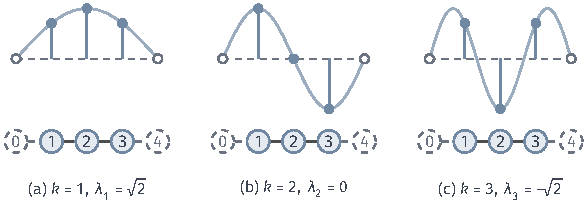
\includegraphics{figures/03-graphs/05-matrices-and-spectra/tikz/adjacency-path-sine-modes/figure.pdf}
  \caption{三点路径$P_3$上的三个正弦特征模式。底部虚线圆圈$0$和$4$为取零值的虚拟边界点，实线圆圈$1,2,3$为路径的实际顶点；上方曲线为$\sin(k\pi t/4)$，蓝色竖杆标出各顶点处的特征向量分量。(a) 基模$k=1$，$\lambda_1=\sqrt{2}$。(b) 二阶模$k=2$，$\lambda_2=0$。(c) 三阶模$k=3$，$\lambda_3=-\sqrt{2}$。}
  \label{fig:adjacency-path-sine-modes}
\end{BookInlineFigure}

\subsection{笛卡儿积图}
\label{sec:adjacency-cartesian-product-spectrum}

许多高维网格和超立方体图都可以由低维简单图通过笛卡儿积拼接而成。设$\mathcal G=(V_{\mathcal G},E_{\mathcal G})$和$\mathcal H=(V_{\mathcal H},E_{\mathcal H})$是两张图，它们的\term{笛卡儿积图}（Cartesian product of graphs）记为$\mathcal G\square\mathcal H$：其顶点集为笛卡儿积$V_{\mathcal G}\times V_{\mathcal H}=\{(u,v):u\in V_{\mathcal G},v\in V_{\mathcal H}\}$，两个顶点对$(u,v)$与$(u',v')$之间有边相连，当且仅当每次恰好沿着一个因子图走一步、另一个坐标保持不变：
\begin{itemize}
\item 要么第二坐标相同（$v=v'$），且第一坐标在$\mathcal G$中相邻（$\{u,u'\}\in E_{\mathcal G}$）；
\item 要么第一坐标相同（$u=u'$），且第二坐标在$\mathcal H$中相邻（$\{v,v'\}\in E_{\mathcal H}$）。
\end{itemize}

图~\ref{fig:adjacency-cartesian-edge-directions}展示了两个单边图$K_2$（顶点为$\{0,1\}$）的笛卡儿积$K_2\square K_2$：四个顶点对$(0,0),(1,0),(1,1),(0,1)$中，蓝色横边只改变第一坐标$u$，绿色竖边只改变第二坐标$v$，对角顶点$(0,0)$与$(1,1)$因同时改变了两个坐标而不相邻，最终围成四元环$C_4$。

\begin{BookInlineFigure}
  \centering
  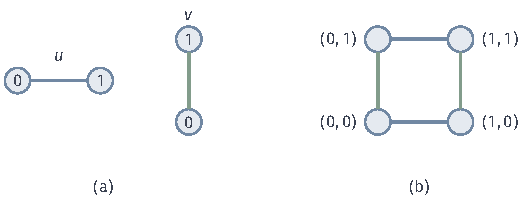
\includegraphics{figures/03-graphs/05-matrices-and-spectra/tikz/adjacency-cartesian-edge-directions/figure.pdf}
  \caption{两个单边图$K_2$的笛卡儿积$K_2\square K_2=C_4$。(a) 两个因子图分别提供第一坐标$u$与第二坐标$v$上的单步移动。(b) 蓝色横边只改变第一坐标$u$，绿色竖边只改变第二坐标$v$，四个顶点对围成四元环。}
  \label{fig:adjacency-cartesian-edge-directions}
\end{BookInlineFigure}

设$\mathcal G$有$p$个顶点、邻接矩阵为$\bm A_{\mathcal G}\in\mathbb R^{p\times p}$，$\mathcal H$有$q$个顶点、邻接矩阵为$\bm A_{\mathcal H}\in\mathbb R^{q\times q}$。按字典序排列$\mathcal G\square\mathcal H$的$pq$个顶点对：第一类边（改变$u$、保持$v$不变）对应的邻接作用是Kronecker积$\bm A_{\mathcal G}\otimes\bm I_q$；第二类边（保持$u$不变、改变$v$）对应的邻接作用是$\bm I_p\otimes\bm A_{\mathcal H}$。两类邻居相加，得到笛卡儿积图的邻接矩阵公式：
\begin{equation}
\bm A_{\mathcal G\square\mathcal H}
=\bm A_{\mathcal G}\otimes\bm I_q+\bm I_p\otimes\bm A_{\mathcal H}.
\label{eq:adjacency-cartesian-product}
\end{equation}

现在设$\bm x\in\mathbb R^p$是$\bm A_{\mathcal G}$属于特征值$\lambda$的特征向量（$\bm A_{\mathcal G}\bm x=\lambda\bm x$），$\bm y\in\mathbb R^q$是$\bm A_{\mathcal H}$属于特征值$\mu$的特征向量（$\bm A_{\mathcal H}\bm y=\mu\bm y$）。考察张量积向量$\bm x\otimes\bm y\in\mathbb R^{pq}$（它在顶点对$(u,v)$处的分量为乘积$x_u y_v$）。利用Kronecker积的混合乘积性质$(\bm M_1\otimes\bm M_2)(\bm x\otimes\bm y)=(\bm M_1\bm x)\otimes(\bm M_2\bm y)$，将$\bm A_{\mathcal G\square\mathcal H}$作用在$\bm x\otimes\bm y$上：
\[
\begin{aligned}
\bm A_{\mathcal G\square\mathcal H}(\bm x\otimes\bm y)
&=(\bm A_{\mathcal G}\bm x)\otimes(\bm I_q\bm y)+(\bm I_p\bm x)\otimes(\bm A_{\mathcal H}\bm y)\\
&=(\lambda\bm x)\otimes\bm y+\bm x\otimes(\mu\bm y)
=(\lambda+\mu)(\bm x\otimes\bm y).
\end{aligned}
\]
这表明$\bm x\otimes\bm y$是$\bm A_{\mathcal G\square\mathcal H}$的特征向量，对应的特征值恰好是两个因子特征值之和$\lambda+\mu$。分别取$\bm A_{\mathcal G}$的$p$个正交特征向量和$\bm A_{\mathcal H}$的$q$个正交特征向量，两两作Kronecker积共得到$pq$个两两正交的特征向量，张成整个$\mathbb R^{pq}$。

\begin{theorem}[笛卡儿积图的邻接谱]
\label{thm:adjacency-cartesian-product-spectrum}
设图$\mathcal G$的全部邻接特征值为$\lambda_1,\ldots,\lambda_p$（对应正交特征基$\bm x_1,\ldots,\bm x_p$），图$\mathcal H$的全部邻接特征值为$\mu_1,\ldots,\mu_q$（对应正交特征基$\bm y_1,\ldots,\bm y_q$）。则笛卡儿积图$\mathcal G\square\mathcal H$的全部$pq$个邻接特征值为两两之和
\[
\bigl\{\lambda_i+\mu_j:1\le i\le p,\;1\le j\le q\bigr\},
\]
其中$\lambda_i+\mu_j$对应的特征向量为$\bm x_i\otimes\bm y_j$。
\end{theorem}

定理~\ref{thm:adjacency-cartesian-product-spectrum}的一个经典应用是计算$d$维超立方体图$Q_d$的谱。$Q_d$的$2^d$个顶点是长度为$d$的$0$--$1$比特串$\{0,1\}^d$，两个比特串相邻当且仅当它们恰好在一个比特位上不同——这正是$d$个单边图$K_2$的连乘笛卡儿积$Q_d=K_2\square K_2\square\cdots\square K_2$。单边图$K_2$的两个特征值为$+1$和$-1$。在$d$个因子中各选一个特征值相加，若有$j$个因子选了$-1$、其余$d-j$个因子选了$+1$，则特征值之和为$(d-j)\cdot 1+j\cdot(-1)=d-2j$。从$d$个因子中挑出$j$个取$-1$共有$\binom{d}{j}$种选法，因此$Q_d$的特征值为$d-2j$（$j=0,1,\ldots,d$），重数为$\binom{d}{j}$。例如三维立方体$Q_3$的$8$个特征值为$3,1,1,1,-1,-1,-1,-3$。

\subsection{正则图的补图}
\label{sec:adjacency-complement-spectrum}

\begin{definition}[正则图]
\label{def:regular-graph}
若简单无向图$\mathcal G$的每个顶点都恰好有$d$个邻居（即所有顶点的度均等于$d$），则称$\mathcal G$为\term{$d$正则图}（$d$-regular graph）。
\end{definition}

在$d$正则图中，邻接矩阵$\bm A$的每一行都有$d$个$1$，行和恒等于$d$。因此给所有顶点统一赋读数$1$时，每个顶点的邻居读数之和都是$d$，即
\[
\bm A\bm 1=d\bm 1.
\]
这说明常向量$\bm 1$必定是$d$正则图属于特征值$d$的特征向量。又因$\bm A$是实对称矩阵，与常向量正交的零和子空间$\bm 1^\perp=\{\bm x\in\mathbb R^n:\bm 1^\top\bm x=0\}$在$\bm A$的作用下保持不变：对任意$\bm x\in\bm 1^\perp$，有$\bm 1^\top(\bm A\bm x)=(\bm A\bm 1)^\top\bm x=d(\bm 1^\top\bm x)=0$。于是我们可以在$\bm 1^\perp$内选出其余$n-1$个正交特征向量$\bm u_2,\ldots,\bm u_n$，这一性质使正则图的补图谱可以直接由原图谱换算出来。

\begin{theorem}[正则图的补图谱]
\label{thm:adjacency-regular-complement}
设$\mathcal G$是$n$个顶点的$d$正则简单无向图，其邻接特征值为$d=\lambda_1\ge\lambda_2\ge\cdots\ge\lambda_n$（其中$\lambda_1=d$对应常向量$\bm 1$，其余$\lambda_2,\ldots,\lambda_n$对应$\bm 1^\perp$中的正交特征向量$\bm u_2,\ldots,\bm u_n$）。则其补图$\overline{\mathcal G}$是$(n-1-d)$正则图，且$\overline{\mathcal G}$的全部邻接特征值为
\[
n-1-d\quad(\text{对应 }\bm 1),
\qquad\text{以及}\qquad
-1-\lambda_i\quad(i=2,\ldots,n,\text{ 对应 }\bm u_i).
\]
\end{theorem}

\begin{proof}
补图$\overline{\mathcal G}$保留相同的顶点集$V$，在所有互异且在原图$\mathcal G$中不相邻的顶点对之间连边。完全图的邻接矩阵为$\bm J-\bm I$，从中减去原图的邻接矩阵$\bm A_{\mathcal G}$，就得到补图的邻接矩阵：
\begin{equation}
\bm A_{\overline{\mathcal G}}=\bm J-\bm I-\bm A_{\mathcal G}.
\label{eq:adjacency-complement-matrix}
\end{equation}

分别考察$\bm A_{\overline{\mathcal G}}$在常向量$\bm 1$和在$\bm u_i\in\bm 1^\perp$（$i=2,\ldots,n$）上的作用：
\begin{itemize}
\item 在常向量$\bm 1$上，$\bm J\bm 1=n\bm 1$且$\bm A_{\mathcal G}\bm 1=d\bm 1$，故
\[
\bm A_{\overline{\mathcal G}}\bm 1=(\bm J-\bm I-\bm A_{\mathcal G})\bm 1=(n-1-d)\bm 1;
\]
\item 对每个$i\in\{2,\ldots,n\}$，因为$\bm u_i\in\bm 1^\perp$，有$\bm J\bm u_i=\bm 1(\bm 1^\top\bm u_i)=\bm 0$，且$\bm A_{\mathcal G}\bm u_i=\lambda_i\bm u_i$，故
\[
\bm A_{\overline{\mathcal G}}\bm u_i=(\bm J-\bm I-\bm A_{\mathcal G})\bm u_i=\bm 0-\bm u_i-\lambda_i\bm u_i=(-1-\lambda_i)\bm u_i.
\]
\end{itemize}
这$n$个正交特征向量给出了$\overline{\mathcal G}$的全部$n$个特征值。注意当原图$\mathcal G$不连通时，部分$i\geq 2$也可能满足$\lambda_i=d$，但由于$\bm u_i\in\bm 1^\perp$，它们在补图中均按$-1-\lambda_i=-1-d$换算。
\end{proof}

以四元环$C_4$（$n=4,d=2$）检验定理~\ref{thm:adjacency-regular-complement}：$C_4$的谱为$\lambda_1=2,\lambda_2=0,\lambda_3=0,\lambda_4=-2$。其补图$\overline{C_4}$只保留两条互不相交的对角边$\{1,3\}$与$\{2,4\}$（即$K_2\sqcup K_2$）。代入换算公式：常向量方向给出$n-1-d=4-1-2=1$；$\bm 1^\perp$中的三个特征值$0,0,-2$依次变为$-1-0=-1$、$-1-0=-1$、$-1-(-2)=1$。补图谱为$\{1,1,-1,-1\}$，与两条独立边各贡献一对$\pm1$完全一致。反之，若原图不是正则图，则$\bm A_{\mathcal G}\bm 1$的各分量是互不相等的顶点度，常向量$\bm 1$不再是$\bm A_{\mathcal G}$的特征向量，$\bm A_{\mathcal G}$与$\bm J$无法在常向量与$\bm 1^\perp$上同时对角化，上述简单换算公式便不再适用。

\section{谱的性质}
\label{sec:adjacency-spectral-properties}

上一节通过直接构造特征向量求出了几类典型图的完整谱。现在回到一般的图，研究邻接谱本身具有哪些普遍的结构性质。我们依次回答四个核心问题：
\begin{enumerate}
\item 最大特征值$\lambda_1$为什么地位特殊？它的重数是多少，对应的特征向量有什么符号特征？
\item 不必解出全部特征值，能否直接用顶点的度给出$\lambda_1$的上下界？
\item 从图中删去边、减小边权或删去顶点后，$\lambda_1$会如何变化？
\item 什么时候正特征值$\lambda$与负特征值$-\lambda$必定成对出现？
\end{enumerate}

本节在非负加权图的一般框架下统一讨论这些问题：设$\bm W=(w_{i,j})\in\mathbb R^{n\times n}$为非负实对称加权邻接矩阵（对角元$w_{i,i}=0$，边权$w_{i,j}=w_{j,i}\geq 0$）；简单无权图的邻接矩阵$\bm A$正是每条边权取$1$的特例。顶点$i$的加权度定义为第$i$行的边权之和$d_i=\sum_{j=1}^n w_{i,j}$。

\subsection{连通图的Perron定理}
\label{sec:adjacency-perron-theorem}

对实对称矩阵$\bm W$，其最大特征值$\lambda_1$可以通过单位球面上的Rayleigh商极值（可参考\BookChapterRef{chap:matrix-approximation}{卷二"矩阵逼近"章}）刻画为
\[
\lambda_1=\max_{\|\bm x\|_2=1}\bm x^\top\bm W\bm x.
\]
为了看清怎样的单位向量$\bm x=(x_1,\ldots,x_n)^\top$能让二次型$\bm x^\top\bm W\bm x$尽可能大，我们把矩阵二次型按图的边展开：
\[
\bm x^\top\bm W\bm x
=\sum_{i=1}^n\sum_{j=1}^n w_{i,j}x_i x_j
=2\sum_{\{i,j\}\in E}w_{i,j}x_i x_j.
\]
这里每一条无向边$\{i,j\}\in E$在双重大和中作为有序对$(i,j)$和$(j,i)$各出现一次，合并贡献$2w_{i,j}x_i x_j$。

观察单条正权边$\{i,j\}$（$w_{i,j}>0$）上的乘积项$2w_{i,j}x_i x_j$：如果两端顶点的赋值$x_i$与$x_j$正负号相反（例如一端取$+1$、另一端取$-1$），乘积$x_i x_j<0$，这条边就会给二次型带来负贡献$-2w_{i,j}|x_i||x_j|$，把总和往小里拉；反之，如果我们把向量$\bm x$的每一个分量都取绝对值，构造非负向量
\[
|\bm x|=\bigl(|x_1|,|x_2|,\ldots,|x_n|\bigr)^\top,
\]
那么一方面向量的欧氏长度完全不变：
\[
\bigl\||\bm x|\bigr\|_2=\sqrt{\sum_{i=1}^n |x_i|^2}=\sqrt{\sum_{i=1}^n x_i^2}=\|\bm x\|_2;
\]
另一方面，由于边权$w_{i,j}\geq 0$，每条边上的乘积都满足$w_{i,j}|x_i||x_j|\geq w_{i,j}x_i x_j$，因此二次型总和只会增大或保持不变：
\[
|\bm x|^\top\bm W|\bm x|
=2\sum_{\{i,j\}\in E}w_{i,j}|x_i||x_j|
\geq 2\sum_{\{i,j\}\in E}w_{i,j}x_i x_j
=\bm x^\top\bm W\bm x.
\]
这意味着：在单位球面上寻找最大化二次型的特征方向时，总可以选到各分量全非负的向量。

图~\ref{fig:adjacency-perron-absolute-value}在三点路径$1\!-\!2\!-\!3$（含两条单位权边$\{1,2\}$和$\{2,3\}$）上直观对比了取绝对值前后的效果。在图~\ref{fig:adjacency-perron-absolute-value}(a)中，取正负交替赋值$\bm x=(1,-1,1)^\top$，两条边的端点乘积均为$x_1x_2=x_2x_3=-1$，二次型为$\bm x^\top\bm A\bm x=2(-1)+2(-1)=-4$，Rayleigh商为$-4/3$；在图~\ref{fig:adjacency-perron-absolute-value}(b)中，逐分量取绝对值得到$|\bm x|=(1,1,1)^\top$，向量长度仍为$\sqrt{3}$，但两条边的端点乘积均变为$+1$，二次型跃升为$|\bm x|^\top\bm A|\bm x|=2(+1)+2(+1)=+4$，Rayleigh商提高到$+4/3$。

\begin{BookInlineFigure}
  \centering
  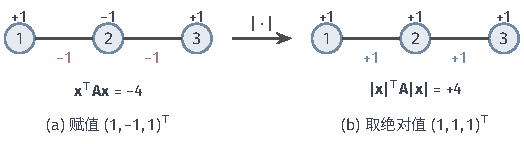
\includegraphics{figures/03-graphs/05-matrices-and-spectra/tikz/adjacency-perron-absolute-value/figure.pdf}
  \caption{三点路径$1\!-\!2\!-\!3$上逐分量取绝对值前后的二次型变化。边下方标注的是端点乘积$x_i x_j$。(a) 赋值$\bm x=(1,-1,1)^\top$时，两条边两端均异号，端点乘积为$-1$，二次型$\bm x^\top\bm A\bm x=2(-1-1)=-4$。(b) 取绝对值得到$|\bm x|=(1,1,1)^\top$后，向量长度不变，每条边的端点乘积变为$+1$，二次型升至$+4$。}
  \label{fig:adjacency-perron-absolute-value}
\end{BookInlineFigure}

在进入正式定理之前，我们先明确加权矩阵$\bm W$的连通条件。在矩阵乘向量$(\bm W\bm x)_i=\sum_{j=1}^n w_{i,j}x_j$中，若两个顶点$i,j$之间的权重$w_{i,j}=0$，则$x_j$对第$i$个输出分量没有任何贡献，二者在矩阵作用中互不相连；只有满足$w_{i,j}>0$的正权边才真正传递数值。为此给出正权支撑的正式定义。

\begin{definition}[正权支撑]
\label{def:positive-weight-support}
设$\bm W=(w_{i,j})\in\mathbb R^{n\times n}$为顶点集$V$上的非负对称邻接权矩阵（对角元$w_{i,i}=0$，边权$w_{i,j}=w_{j,i}\geq 0$）。保留全体顶点$V$、仅保留严格正权边
\begin{equation}
E_+=\bigl\{\{i,j\}\subseteq V:w_{i,j}>0\bigr\}
\label{eq:positive-weight-support}
\end{equation}
所构成的无权简单图$\mathcal G_+=(V,E_+)$称为加权图（或矩阵$\bm W$）的\term{正权支撑}（positive-weight support）。
\end{definition}

当正权支撑$\mathcal G_+$连通时，任意两个顶点之间都存在一条每步边权均严格大于零的路径，非零读数才能沿正权路径传遍全图所有顶点。

\begin{theorem}[连通图的Perron定理]
\label{thm:adjacency-perron}
设$\bm W=(w_{i,j})\in\mathbb R^{n\times n}$为有限无向图的非负对称邻接权矩阵，且其正权支撑$\mathcal G_+$连通（$n\geq 2$）。则：
\begin{enumerate}
\item 最大特征值$\lambda_1>0$的代数重数为$1$，且存在各分量均严格为正的特征向量$\bm p=(p_1,\ldots,p_n)^\top$（$p_i>0,\forall i$）；
\item $\bm W$的任意特征值$\lambda$均满足$|\lambda|\leq\lambda_1$（即谱半径等于$\lambda_1$）。
\end{enumerate}
\end{theorem}

\begin{proof}
我们分三步依次证明：（1）存在各分量严格为正的最大特征向量$\bm p$；（2）最大特征值$\lambda_1$的特征空间是一维的（重数为$1$）；（3）其余特征值均满足$|\lambda|\leq\lambda_1$。

\textbf{第一步（严格正特征向量的存在性）}：在单位球面$\|\bm x\|_2=1$上任取一个使Rayleigh商达到最大值$\lambda_1$的单位特征向量$\bm x$，令$\bm p=|\bm x|$。由前面的绝对值不等式，有
\[
\lambda_1\geq\bm p^\top\bm W\bm p
=\sum_{i,j}w_{i,j}|x_i||x_j|
\geq\sum_{i,j}w_{i,j}x_i x_j
=\bm x^\top\bm W\bm x=\lambda_1,
\]
且$\|\bm p\|_2=\|\bm x\|_2=1$。因此$\bm p^\top\bm W\bm p=\lambda_1$，即非负单位向量$\bm p$也在单位球面上达到最大Rayleigh商$\lambda_1$。由Rayleigh商在极值点处的驻点条件，$\bm p$本身就是属于最大特征值$\lambda_1$的特征向量：$\bm W\bm p=\lambda_1\bm p$。又因正权支撑连通且$n\geq 2$，图中至少有一条正权边，取常向量即可见$\lambda_1>0$。

下面用反证法说明$\bm p$不可能含有零分量。假设存在某个顶点$i$使得$p_i=0$。读取特征方程$\bm W\bm p=\lambda_1\bm p$的第$i$行：
\[
0=\lambda_1 p_i=\sum_{j=1}^n w_{i,j}p_j.
\]
由于右端每一项都满足$w_{i,j}\geq 0$且$p_j\geq 0$，非负项之和等于零迫使每一项都等于零。特别地，对顶点$i$在正权支撑中的每一个邻居$j$（满足$w_{i,j}>0$），都必有$p_j=0$。也就是说，“分量为零”这一性质会从顶点$i$传播到它的所有正权邻居。由于正权支撑$\mathcal G_+$连通，从$i$出发沿正权路径逐歩传递，最终推出全图所有顶点的分量都满足$p_k=0$（$\forall k\in V$），即$\bm p=\bm 0$，这与$\|\bm p\|_2=1$矛盾。因此$\bm p$的每个分量都严格为正：$p_i>0$（$\forall i\in V$）。

\textbf{第二步（$\lambda_1$的重数为$1$）}：用反证法。假设$\lambda_1$的特征子空间维数大于$1$，则可以在该特征子空间中选出一个与$\bm p$正交的单位特征向量$\bm y$（满足$\bm W\bm y=\lambda_1\bm y$，$\|\bm y\|_2=1$，且$\langle\bm p,\bm y\rangle=0$）。

对$\bm y$重复第一步的推导：令$|\bm y|=(|y_1|,\ldots,|y_n|)^\top$，则$|\bm y|$也是属于$\lambda_1$的非负单位特征向量；再由第一步的零分量传播论证，可知$|\bm y|$的每个分量都严格为正，从而$\bm y$的每个分量都非零（$y_i\neq 0,\forall i\in V$）。

另一方面，由于$|\bm y|^\top\bm W|\bm y|=\bm y^\top\bm W\bm y=\lambda_1$，不等式
\[
\sum_{\{i,j\}\in E}2w_{i,j}|y_i||y_j|
\geq\sum_{\{i,j\}\in E}2w_{i,j}y_i y_j
\]
必须取等号。因为每一条边上的差$2w_{i,j}(|y_i||y_j|-y_i y_j)\geq 0$都非负，总和为零要求每一条正权边$\{i,j\}\in E_+$（$w_{i,j}>0$）都满足$|y_i||y_j|=y_i y_j$。由于$y_i\neq 0$且$y_j\neq 0$，这意味着正权边的两个端点$y_i$与$y_j$必须严格同号。沿连通的正权支撑传递，向量$\bm y$的所有$n$个分量必定同为正数或同为负数。然而$\bm p$的所有分量严格为正，于是内积$\langle\bm p,\bm y\rangle=\sum_{i=1}^n p_i y_i$是$n$个严格同号非零项之和，绝不可能等于$0$——这与$\langle\bm p,\bm y\rangle=0$矛盾。故$\lambda_1$的特征空间只能是一维的，重数为$1$。

\textbf{第三步（谱半径界$|\lambda|\leq\lambda_1$）}：任取$\bm W$的一个特征值$\lambda$及其单位特征向量$\bm z$（$\|\bm z\|_2=1$）。由三角不等式与$\lambda_1$的极大性质，
\[
|\lambda|
=|\bm z^\top\bm W\bm z|
=\Bigl|\sum_{i,j}w_{i,j}z_i z_j\Bigr|
\leq\sum_{i,j}w_{i,j}|z_i||z_j|
=|\bm z|^\top\bm W|\bm z|
\leq\lambda_1,
\]
定理证毕。
\end{proof}

定理~\ref{thm:adjacency-perron}中唯一确定的严格正单位特征向量$\bm p$称为图的\term{Perron向量}（Perron vector）。需要注意，定理保证最大特征值$\lambda_1$本身是单根，但并不排除最小特征值$\lambda_n$达到相反数$-\lambda_1$（此时$|\lambda_n|=\lambda_1$）。例如单边图$K_2$的特征值为$+1$和$-1$。第~\ref{sec:adjacency-bipartite-symmetry}小节将证明：在正权支撑连通图上，$\lambda_n=-\lambda_1$发生当且仅当该图是二部图。

\subsection{谱的上下界}
\label{sec:adjacency-degree-bounds}

Perron定理确立了最大特征值$\lambda_1$的单根性与正特征向量，但在一般非正则图上并不能直接写出$\lambda_1$的闭式解。下面我们分别利用Rayleigh商的下界性质和Perron向量的最大分量，证明$\lambda_1$始终被夹在图的平均度$\overline d$与最大度$d_{\max}$之间。

\paragraph{下界：用全一常向量测试Rayleigh商}

根据Rayleigh商的极大性质，最大特征值$\lambda_1$是$\frac{\bm x^\top\bm W\bm x}{\bm x^\top\bm x}$在所有非零向量$\bm x\neq\bm 0$上的最大值：
\[
\lambda_1=\max_{\bm x\neq\bm 0}\frac{\bm x^\top\bm W\bm x}{\bm x^\top\bm x}.
\]
因此，我们随便挑选一个具体的非零向量$\bm x$代进去算出的Rayleigh商，都必然小于或等于最大值$\lambda_1$。

取最简单的全一常向量$\bm x=\bm 1=(1,1,\ldots,1)^\top\in\mathbb R^n$（所有顶点赋相同的读数$1$），分两步计算它的Rayleigh商。先算矩阵乘向量$\bm W\bm 1$：按矩阵乘法规则，$\bm W\bm 1$的第$i$个分量是把$\bm W$第$i$行的所有元素各自乘以$1$再相加：
\[
(\bm W\bm 1)_i=\sum_{j=1}^n w_{i,j}\cdot 1=\sum_{j=1}^n w_{i,j}=d_i.
\]
也就是说，对全一向量$\bm 1$作用一次邻接矩阵$\bm W$，输出向量的第$i$个分量恰好就是顶点$i$的加权度$d_i$，即$\bm W\bm 1=(d_1,d_2,\ldots,d_n)^\top$（若改用单位化常向量$\bm u=\frac{1}{\sqrt n}\bm 1$，则输出的第$i$个分量为$d_i/\sqrt n$）。

再算二次型与Rayleigh商：用行向量$\bm 1^\top$左乘输出向量$\bm W\bm 1$，相当于把全部$n$个顶点的度相加：
\[
\bm 1^\top\bm W\bm 1=\sum_{i=1}^n 1\cdot(\bm W\bm 1)_i=\sum_{i=1}^n d_i.
\]
而全一向量本身的长度平方为$\bm 1^\top\bm 1=\sum_{i=1}^n 1^2=n$。将两者相除，就得到全一向量$\bm 1$的Rayleigh商恰好等于全图的平均度$\overline d$：
\[
\frac{\bm 1^\top\bm W\bm 1}{\bm 1^\top\bm 1}
=\frac{1}{n}\sum_{i=1}^n d_i
=\overline d.
\]
在简单无权图中，每条无向边为两个端点的度各贡献$1$，总度数$\sum_{i=1}^n d_i=2m$，故平均度为$\overline d=2m/n$。由于最大值$\lambda_1$不小于特定向量$\bm 1$的Rayleigh商，立即得到下界：
\[
\lambda_1\geq\overline d.
\]

\paragraph{上界：在Perron向量的最大分量处放缩}

再证上界$\lambda_1\leq d_{\max}$，其中$d_{\max}=\max_{1\leq i\leq n}d_i$为全图的最大度。取属于$\lambda_1$的非负特征向量$\bm p=(p_1,\ldots,p_n)^\top\neq\bm 0$（连通图上即为严格正的Perron向量），并在全部$n$个顶点中找出分量最大的那个顶点$i^\star$，使得
\[
p_{i^\star}=\max_{1\leq j\leq n}p_j>0.
\]
写出特征方程$\bm W\bm p=\lambda_1\bm p$在顶点$i^\star$这一行的等式，并将右端每个邻居的分量$p_j$放大为最大值$p_{i^\star}$（注意到$w_{i^\star,j}\geq 0$）：
\[
\lambda_1 p_{i^\star}
=\sum_{j=1}^n w_{i^\star,j}\,p_j
\leq\sum_{j=1}^n w_{i^\star,j}\,p_{i^\star}
=\Bigl(\sum_{j=1}^n w_{i^\star,j}\Bigr)p_{i^\star}
=d_{i^\star}\,p_{i^\star}
\leq d_{\max}\,p_{i^\star}.
\]
因为$p_{i^\star}>0$，在不等式两端同除以正数$p_{i^\star}$，即得上界$\lambda_1\leq d_{\max}$。

\begin{theorem}[最大邻接特征值的度界]
\label{prop:adjacency-degree-bounds}
对任意非负实对称邻接矩阵$\bm W\in\mathbb R^{n\times n}$，其最大特征值$\lambda_1$满足
\begin{equation}
\overline d\leq\lambda_1\leq d_{\max}.
\label{eq:adjacency-degree-spectral-bounds}
\end{equation}
若$\bm W$的正权支撑连通，则$\lambda_1=\overline d$（或$\lambda_1=d_{\max}$）成立当且仅当图中所有顶点的加权度均相等（即图为正则图）。
\end{theorem}

\paragraph{取等条件}

我们来追踪正权支撑连通时式~\eqref{eq:adjacency-degree-spectral-bounds}两端何时取等号。若上界$\lambda_1=d_{\max}$取等，则前面关于最大分量顶点$i^\star$的两步放缩必须同时取等号：第一步等号$\sum_j w_{i^\star,j}(p_{i^\star}-p_j)=0$要求$i^\star$的每一个正权邻居$j$（$w_{i^\star,j}>0$）都达到最大分量$p_j=p_{i^\star}$，第二步等号要求$d_{i^\star}=d_{\max}$。既然正权邻居$j$也达到了最大分量$p_j=p_{i^\star}$，对顶点$j$再次应用同样的推理，可知$d_j=d_{\max}$且$j$的所有正权邻居分量也等于$p_{i^\star}$。沿连通的正权支撑传遍全图，所有顶点的度都必须等于$d_{\max}$，图必为正则图。

若下界$\lambda_1=\overline d$取等，则说明常向量$\bm 1$的Rayleigh商已经达到了全局最大值$\lambda_1$，因此$\bm 1$本身就是属于$\lambda_1$的特征向量，满足$\bm W\bm 1=\overline d\,\bm 1$。逐分量读取该式，即得对所有顶点$i$都有$d_i=(\bm W\bm 1)_i=\overline d$，图同样是正则图。

以三点路径$P_3$和四点环$C_4$对照：$P_3$的度序列为$(1,2,1)$，平均度$\overline d=4/3\approx 1.333$，最大特征值$\lambda_1=\sqrt 2\approx 1.414$，最大度$d_{\max}=2$，满足严格不等式$4/3<\sqrt 2<2$；而$2$正则图$C_4$的度序列为$(2,2,2,2)$，三者相等$\overline d=\lambda_1=d_{\max}=2$。

\subsection{子图的谱单调性}
\label{sec:adjacency-spectral-monotonicity}

如果在图中删去一条边、降低某条边的正权重，或者删去一个顶点及其关联边，每个顶点的邻居贡献只减不增。下面用非负最大化向量证明：最大特征值$\lambda_1$对子图具有单调性，且在连通图上删去任何正权边或顶点都会使$\lambda_1$严格下降。

设$\bm W'\in\mathbb R^{n\times n}$是由$\bm W\in\mathbb R^{n\times n}$减小部分边权（包括将边权降为$0$以表示删边，或将某个被删顶点的整行整列置为$0$）所得的非负对称矩阵，满足逐元素$0\leq w'_{i,j}\leq w_{i,j}$。在$\bm W'$上取一个非负单位特征向量$\bm x\geq\bm 0$（$\|\bm x\|_2=1$）使得$\bm x^\top\bm W'\bm x=\lambda_1(\bm W')$。将同一个非负单位向量$\bm x$代入原矩阵$\bm W$的二次型比较：
\[
\lambda_1(\bm W')
=\bm x^\top\bm W'\bm x
=\sum_{i,j}w'_{i,j}x_i x_j
\leq\sum_{i,j}w_{i,j}x_i x_j
=\bm x^\top\bm W\bm x
\leq\lambda_1(\bm W).
\]
这里第一个不等式来自$0\leq w'_{i,j}\leq w_{i,j}$与$x_i x_j\geq 0$，第二个不等式来自$\lambda_1(\bm W)$是$\bm W$在单位球面上的最大Rayleigh商。

进一步，若原图$\bm W$的正权支撑连通，且$\bm W'\neq\bm W$（确实减小了至少一条边$\{u,v\}$的权重$w'_{u,v}<w_{u,v}$），能否出现等号$\lambda_1(\bm W')=\lambda_1(\bm W)$？若两端相等，则上面不等式链中的两处不等号都必须取等：一方面，第二处取等$\bm x^\top\bm W\bm x=\lambda_1(\bm W)$说明$\bm x$也是连通矩阵$\bm W$达到$\lambda_1(\bm W)$的单位特征向量，由定理~\ref{thm:adjacency-perron}（Perron定理）知$\bm x$的每一个分量都严格为正（$x_i>0,\forall i\in V$）；另一方面，既然$x_u>0$且$x_v>0$，在权重严格减小的那条边$\{u,v\}$上就有$w'_{u,v}x_u x_v<w_{u,v}x_u x_v$，导致第一处不等式严格成立$\bm x^\top\bm W'\bm x<\bm x^\top\bm W\bm x$，产生矛盾。因此，在正权支撑连通图上，删去任意正权边、降低任意正权边的权重，或删去任意顶点，都会使最大邻接特征值严格减小：$\lambda_1(\bm W')<\lambda_1(\bm W)$。

例如从$n$点环$C_n$中删去一条边得到路径$P_n$，最大特征值从$\lambda_1(C_n)=2$严格下降为$\lambda_1(P_n)=2\cos\bigl(\frac{\pi}{n+1}\bigr)<2$。反之，若原图不连通，例如取$\mathcal G=C_4\sqcup K_2$，其最大特征值$\lambda_1=2$由$C_4$分量单独决定；此时删去较小分量$K_2$中的边并不会改变全图的最大特征值$\lambda_1=2$，这说明严格单调性确实依赖原图的连通性假设。

\subsection{二部图的谱对称性}
\label{sec:adjacency-bipartite-symmetry}

前面三小节聚焦于谱右端的最大特征值$\lambda_1$。现在我们把目光转向整个邻接谱的左右两端：在什么条件下，图的邻接谱关于原点对称（即每个特征值$\lambda$与$-\lambda$以相同重数成对出现）？答案恰好刻画了二部图。

先看二部图为什么必然具有对称谱。设图$\mathcal G$是二部图，其顶点集划分为左右两个独立集$V=X\cup Y$，所有正权边都横跨在$X$与$Y$之间（同侧内部没有任何正权边）。我们构造一个$n\times n$对角符号矩阵$\bm S=\operatorname{diag}(s_1,\ldots,s_n)$：
\[
s_i=
\begin{cases}
+1,& i\in X,\\
-1,& i\in Y.
\end{cases}
\]
显然$\bm S^\top=\bm S$且$\bm S^2=\bm I$（$\bm S$是正交对合矩阵）。考察正交相似变换$\bm S\bm W\bm S$的第$(i,j)$个元素$s_i w_{i,j}s_j$：当$w_{i,j}>0$时，边$\{i,j\}$连接$X$与$Y$异侧端点，必有$s_i s_j=(+1)(-1)=-1$，故$s_i w_{i,j}s_j=-w_{i,j}$；当$w_{i,j}=0$时，同样有$s_i w_{i,j}s_j=0=-w_{i,j}$。因此，对角符号矩阵$\bm S$把整个邻接权矩阵$\bm W$变成了它的相反数：
\begin{equation}
\bm S\bm W\bm S=-\bm W,\qquad\text{或等价地}\qquad \bm W\bm S=-\bm S\bm W.
\label{eq:adjacency-bipartite-anticommute}
\end{equation}

利用式~\eqref{eq:adjacency-bipartite-anticommute}，若$\bm x$是$\bm W$属于特征值$\lambda$的特征向量（$\bm W\bm x=\lambda\bm x$），将$\bm W$作用在翻转了$Y$侧符号的向量$\bm S\bm x$上：
\[
\bm W(\bm S\bm x)=-\bm S\bm W\bm x=-\bm S(\lambda\bm x)=(-\lambda)(\bm S\bm x).
\]
这表明$\bm S\bm x$正是$\bm W$属于相反数特征值$-\lambda$的特征向量。图~\ref{fig:adjacency-bipartite-sign-flip}在四元环$C_4$（二部划分$X=\{1,3\},Y=\{2,4\}$）上展示了这一操作：将属于$\lambda=+2$的特征向量$\bm x=(1,1,1,1)^\top$在$Y$侧变号，立即得到属于$-\lambda=-2$的特征向量$\bm S\bm x=(1,-1,1,-1)^\top$。由于可逆矩阵$\bm S$在$\lambda$的特征子空间与$-\lambda$的特征子空间之间建立了线性同构，两个特征值$\lambda$与$-\lambda$的代数重数必然完全相等，即整个邻接谱关于原点对称：$\lambda_i=-\lambda_{n+1-i}$（$i=1,\ldots,n$）。

\begin{BookInlineFigure}
  \centering
  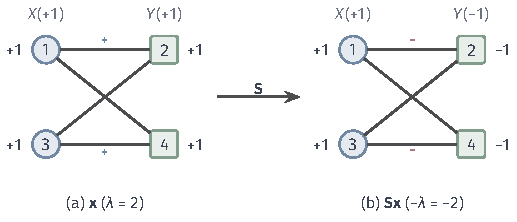
\includegraphics{figures/03-graphs/05-matrices-and-spectra/tikz/adjacency-bipartite-sign-flip/figure.pdf}
  \caption{二部图上的对角符号翻转$\bm S\bm W\bm S=-\bm W$（以$C_4$为例，圆点为$X=\{1,3\}$，方点为$Y=\{2,4\}$）。(a) 属于特征值$\lambda=+2$的特征向量$\bm x=(1,1,1,1)^\top$，跨部边两端同号。(b) 经$\bm S$保持$X$侧符号、翻转$Y$侧符号后，跨部边两端全部反号，得到属于特征值$-\lambda=-2$的特征向量$\bm S\bm x=(1,-1,1,-1)^\top$。}
  \label{fig:adjacency-bipartite-sign-flip}
\end{BookInlineFigure}

反过来，谱关于原点对称（甚至在连通图上仅最小特征值满足$\lambda_n=-\lambda_1$）也能反推出图是二部图。

\begin{theorem}[二部图的谱对称性]
\label{thm:adjacency-bipartite-spectral-symmetry}
设$\bm W\in\mathbb R^{n\times n}$为有限无向无自环图的非负对称邻接权矩阵。则以下命题成立：
\begin{enumerate}
\item $\bm W$的邻接谱关于零对称（即对每个$i=1,\ldots,n$都有$\lambda_i=-\lambda_{n+1-i}$），当且仅当其正权支撑$\mathcal G_+$是二部图（不含奇数长度的环）；
\item 若进一步$\bm W$的正权支撑连通且$n\geq 2$，则只需两端特征值满足$\lambda_n=-\lambda_1$，即可判定正权支撑$\mathcal G_+$是二部图。
\end{enumerate}
\end{theorem}

\begin{proof}
\textbf{第1条}：充分性（二部图$\implies$谱关于零对称）已由式~\eqref{eq:adjacency-bipartite-anticommute}给出。下面证明必要性（谱关于零对称$\implies$不含奇环）：若邻接谱关于零对称，则对任意正奇数$k=1,3,5,\ldots$，每一对相反特征值$\lambda$与$-\lambda$的奇数次幂滿足$(-\lambda)^k=-\lambda^k$，相加相互抵消（零特征值的幂本身为$0$），因此所有奇数阶谱矩恒等于零：
\[
\operatorname{tr}(\bm W^k)=\sum_{i=1}^n\lambda_i^k=0,\qquad k=1,3,5,\ldots.
\]
假设正权支撑$\mathcal G_+$中含有一个奇数长度$\ell$的简单环$v_1\to v_2\to\cdots\to v_\ell\to v_1$。沿该奇环绕行一圈是一条长度为$\ell$的闭行走，其沿途每一步的边权均严格为正，乘积$w_{v_1,v_2}w_{v_2,v_3}\cdots w_{v_\ell,v_1}>0$为$(\bm W^\ell)_{v_1,v_1}$贡献了一个严格正数。由于$\bm W$的所有元素非负，其余一切$\ell$步闭行走的权重乘积均非负，不可能抵消这一正贡献，从而$\operatorname{tr}(\bm W^\ell)>0$，与奇数阶迹为零矛盾。故正权支撑$\mathcal G_+$中不含奇环，必为二部图。

\textbf{第2条}：设正权支撑$\mathcal G_+$连通（$n\geq 2$，从而$\lambda_1>0$）且$\lambda_n=-\lambda_1$。取属于最小特征值$\lambda_n$的实单位特征向量$\bm x$（$\bm W\bm x=\lambda_n\bm x$，$\|\bm x\|_2=1$），则$\bm x^\top\bm W\bm x=\lambda_n=-\lambda_1$。考察绝对值向量$|\bm x|=(|x_1|,\ldots,|x_n|)^\top$的二次型：
\[
\begin{aligned}
\lambda_1
&\geq|\bm x|^\top\bm W|\bm x|
=\sum_{i,j}w_{i,j}|x_i||x_j|
\geq\Bigl|\sum_{i,j}w_{i,j}x_i x_j\Bigr|\\
&=|\bm x^\top\bm W\bm x|
=-\bm x^\top\bm W\bm x
=-\lambda_n=\lambda_1.
\end{aligned}
\]
首尾两端相等迫使中间不等式全部取等号。首先，$|\bm x|^\top\bm W|\bm x|=\lambda_1$说明非负单位向量$|\bm x|$达到了最大特征值$\lambda_1$；由定理~\ref{thm:adjacency-perron}（Perron定理），$|\bm x|$是严格正的Perron向量，故$|x_i|>0$（即$x_i\neq 0,\forall i\in V$）。其次，$\sum_{i,j}w_{i,j}|x_i||x_j|=\sum_{i,j}w_{i,j}(-x_i x_j)$等价于
\[
\sum_{\{i,j\}\in E_+}2w_{i,j}\bigl(|x_i||x_j|+x_i x_j\bigr)=0.
\]
由于对每条边都有$|x_i||x_j|+x_i x_j\geq 0$且正权边满足$w_{i,j}>0$，每一条正权边$\{i,j\}\in E_+$都必须满足
\[
x_i x_j=-|x_i||x_j|<0.
\]
这意味着：每条正权边的两个端点在向量$\bm x$中的分量符号必定一正一负。令
\[
X=\{i\in V:x_i>0\},\qquad Y=\{i\in V:x_i<0\},
\]
由于每个$x_i\neq 0$，$V=X\cup Y$构成顶点集的一个划分，且所有正权边都连接$X$中的顶点与$Y$中的顶点，$X$与$Y$内部均无正权边。因此正权支撑$\mathcal G_+$是二部图。
\end{proof}

对比两个例子：四元环$C_4$的谱为$\{2,0,0,-2\}$，关于零对称且$\lambda_4=-2=-\lambda_1$，是二部图；三角形$C_3$的谱为$\{2,-1,-1\}$，不关于零对称且$\lambda_3=-1\neq -\lambda_1$，含有奇环。同时要注意第2条中“正权支撑连通”这一前提不可省略：若取不连通图$\mathcal G=C_3\sqcup K_{3,3}$，其中$C_3$的谱为$\{2,-1,-1\}$、二部图分量$K_{3,3}$的谱为$\{3,0,0,0,0,-3\}$，合在一起全图最大特征值$\lambda_1=3$与最小特征值$\lambda_9=-3$依然满足$\lambda_9=-\lambda_1$，但整张图因包含三角形分量$C_3$而不是二部图（此时完整谱中由$C_3$贡献的$+2$没有对应的$-2$，按第1条的完整谱对称性仍能准确排除二部性）。

\section{图结构的谱刻画}
\label{sec:adjacency-spectral-structure}

如果只知道一张简单无向图$\mathcal G=(V,E)$的邻接谱$\lambda_1\ge\lambda_2\ge\cdots\ge\lambda_n$，我们能从中恢复出哪些图的结构参数，又能对哪些组合不变量给出上下界？

本节从局部到全局依次展开：第~\ref{sec:adjacency-low-spectral-moments}小节由二阶、三阶谱矩计数边和三角形，并结合顶点度从四阶谱矩计算四环数；第~\ref{sec:adjacency-diameter-bound}小节利用矩阵幂的线性无关性证明不同特征值的个数至少比图的直径多$1$；第~\ref{sec:adjacency-chromatic-bounds}小节结合导出子图的谱交错性质与单位根相位消去法，给出图色数$\chi(\mathcal G)$的谱上下界；第~\ref{sec:adjacency-hoffman-independence}小节通过中心化指示向量的Rayleigh商导出正则图最大独立集$\alpha(\mathcal G)$的Hoffman上界；最后，第~\ref{sec:adjacency-spectral-information}小节通过同谱非同构图反例，总结完整邻接谱的信息边界。

\subsection{局部结构}
\label{sec:adjacency-low-spectral-moments}

设简单无向图$\mathcal G=(V,E)$有$n=|V|$个顶点、$m=|E|$条边，顶点$v$的度记为$d_v$。由第~\ref{sec:adjacency-walk-counts}节的谱矩公式~\eqref{eq:adjacency-spectral-moments}，第$k$阶谱矩$\sum_{i=1}^n\lambda_i^k=\operatorname{tr}(\bm A^k)$等于全图长度为$k$的闭行走总数。当$k=1$时，简单无向图没有自环，一步闭行走条数为零，故一阶谱矩恒为$\operatorname{tr}(\bm A)=\sum_{i=1}^n\lambda_i=0$。下面依次分析$k=2,3,4$时的闭行走与局部子图计数。

\paragraph{边数}

考察长度为$2$的闭行走$u\to z\to u$。由于步数只有两步，第一步从起点$u$走到某个邻居$z$，第二步必须沿同一条边$\{u,z\}$原路退回$u$。因此，对顶点$u$的每一个邻居$z$，都恰好有一条两步闭行走$u\to z\to u$，从而对角元$(\bm A^2)_{u,u}=d_u$就是顶点$u$的度。

如图~\ref{fig:adjacency-edge-triangle-walks}(a)(b)所示，图中的每一条无向边$\{u,v\}\in E$恰好对应两条起点不同的两步闭行走：$u\to v\to u$（计入$(\bm A^2)_{u,u}$）和$v\to u\to v$（计入$(\bm A^2)_{v,v}$）。全图共有$m$条边，故两步闭行走总数为$2m$：
\[
\operatorname{tr}(\bm A^2)=\sum_{u\in V}d_u=\sum_{i=1}^n\lambda_i^2=2m.
\]

\paragraph{三角形数}

考察长度为$3$的闭行走$u\to v\to w\to u$。因为简单图没有自环，相邻两步的顶点必定互不相同（$v\neq u$，$w\neq v$，$u\neq w$），所以途中经过的三个顶点$u,v,w$必然两两互异，且两两之间都有边相连——它们在图中恰好围成一个三角形（三元环$C_3$）。

每一个三角形$\{u,v,w\}$会贡献多少条三步闭行走？如图~\ref{fig:adjacency-edge-triangle-walks}(c)(d)所示，固定一个起点$u$后，可以按$u\to v\to w\to u$和$u\to w\to v\to u$两个相反方向绕行，给出$2$条三步闭行走；三角形共有$3$个顶点可作为起点，每个起点各有$2$个绕行方向，因此每一个三角形恰好产生$3\times 2=6$条三步闭行走。

\begin{BookInlineFigure}
  \centering
  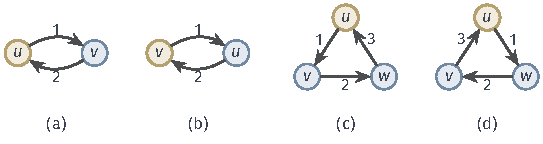
\includegraphics{figures/03-graphs/05-matrices-and-spectra/tikz/adjacency-edge-triangle-walks/figure.pdf}
  \caption{简单图上的两步与三步闭行走计数。浅黄色顶点标出闭行走的起点，箭头旁数字为步序。(a)(b) 同一条无向边$\{u,v\}$分别以$u$和$v$为起点各产生一条两步往返闭行走，共$2$条。(c)(d) 同一个三角形$\{u,v,w\}$在固定起点$u$下有顺、逆两个绕行方向；换遍三个起点共产生$3\times 2=6$条三步闭行走。}
  \label{fig:adjacency-edge-triangle-walks}
\end{BookInlineFigure}

记$t_3$为图$\mathcal G$中三角形（无序三元子集）的个数，则全图三步闭行走总数为$6t_3$。由此，图的边数$m$与三角形个数$t_3$可完全由二阶与三阶谱矩直接算出：
\begin{equation}
m=\frac12\operatorname{tr}(\bm A^2)=\frac12\sum_{i=1}^n\lambda_i^2,
\qquad
t_3=\frac16\operatorname{tr}(\bm A^3)=\frac16\sum_{i=1}^n\lambda_i^3.
\label{eq:adjacency-edge-triangle-counts}
\end{equation}

我们在四点环加对角边$\{1,3\}$的图上核对式~\eqref{eq:adjacency-edge-triangle-counts}。该图有$n=4$个顶点、$m=5$条边和$t_3=2$个三角形（即$\{1,2,3\}$与$\{1,3,4\}$）。其邻接矩阵$\bm A$与平方$\bm A^2$分别为
\[
\bm A=
\begin{bmatrix}
0&1&1&1\\
1&0&1&0\\
1&1&0&1\\
1&0&1&0
\end{bmatrix},
\qquad
\bm A^2=
\begin{bmatrix}
3&1&2&1\\
1&2&1&2\\
2&1&3&1\\
1&2&1&2
\end{bmatrix}.
\]
读取$\bm A^2$的四个对角元$(3,2,3,2)$，恰好是四个顶点的度$(d_1,d_2,d_3,d_4)$，二阶迹为$\operatorname{tr}(\bm A^2)=3+2+3+2=10$，除以$2$得边数$m=10/2=5$。再算$\bm A^3=\bm A^2\bm A$的对角元：例如$(\bm A^3)_{1,1}$是$\bm A^2$的第一行$(3,1,2,1)$与$\bm A$的第一列$(0,1,1,1)^\top$的内积，等于$1+2+1=4$（对应经过顶点$1$的两个三角形各贡献$2$个绕行方向）；同理可得$\bm A^3$的四个对角元为$(4,2,4,2)$，三阶迹为$\operatorname{tr}(\bm A^3)=4+2+4+2=12$，除以$6$得三角形数$t_3=12/6=2$。

\paragraph{四环数}

到了$k=4$步闭行走$v_0\to v_1\to v_2\to v_3\to v_0$，由于闭行走既可以沿简单四元环绕行，也可以在单条边或相邻两条边上来回折返，四阶谱矩$\operatorname{tr}(\bm A^4)$不再只包含四元环。按一条四步闭行走途中实际访问的不同顶点个数，可以将其不重不漏地分为三类（图~\ref{fig:adjacency-four-step-walks}）：
\begin{enumerate}
\item \textbf{第一类（只经过$2$个不同顶点）}：如图~\ref{fig:adjacency-four-step-walks}(a)所示，四步始终在同一条边$\{u,v\}$上来回折返两次。每条边有$u\to v\to u\to v\to u$和$v\to u\to v\to u\to v$两条记录，全图$m$条边共贡献$2m$条闭行走。
\item \textbf{第二类（经过$3$个不同顶点）}：如图~\ref{fig:adjacency-four-step-walks}(b)所示，在四个步序位置$v_0,v_1,v_2,v_3$中，必有某一个中心顶点$v$出现了两次，另外两个顶点$a,b$各出现一次（因无自环，重复顶点$v$只能隔一步出现在$v_0,v_2$或$v_1,v_3$位置，且$a,b$均与中心点$v$相邻，构成长为$2$的星形分支$a\text{--}v\text{--}b$）。对固定的一对公共邻居$\{a,b\}\subseteq N(v)$，共有$4$条四步闭行走：从中心$v$出发的$v\to a\to v\to b\to v$和$v\to b\to v\to a\to v$（$2$条），从端点$a$出发的$a\to v\to b\to v\to a$（$1$条），以及从端点$b$出发的$b\to v\to a\to v\to b$（$1$条）。在每个顶点$v\in V$处，从其$d_v$个邻居中选出一对无序邻居$\{a,b\}$共有$\binom{d_v}{2}$种选法，因此第二类闭行走总数为$4\sum_{v\in V}\binom{d_v}{2}$。
\item \textbf{第三类（经过$4$个不同顶点）}：如图~\ref{fig:adjacency-four-step-walks}(c)所示，四个顶点互不重复，首尾相连围成一个简单四元环$C_4$。设图中四元环的个数为$t_4$，每个四元环有$4$个可选起点、每个起点有顺逆$2$个绕行方向，共贡献$8t_4$条闭行走。
\end{enumerate}

\begin{BookInlineFigure}
  \centering
  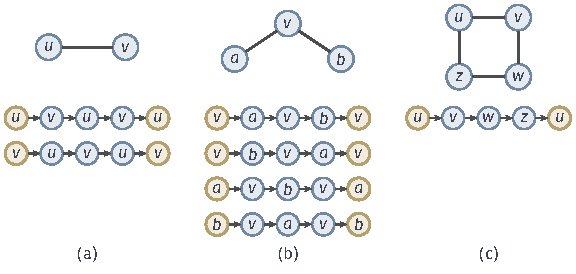
\includegraphics{figures/03-graphs/05-matrices-and-spectra/tikz/adjacency-four-step-walks/figure.pdf}
  \caption{按途中访问的不同顶点个数对四步闭行走分类。上排画出所使用的边，下排每一行从左到右列出一条五点访问序列，浅黄色标出重合的起点与终点。(a) 仅用$2$个顶点：在同一条边上来回折返两次（每条边$2$条）。(b) 使用$3$个顶点：在共享端点$v$的两条相邻边上各往返一次（每对相邻边$4$条）。(c) 使用$4$个不同顶点：沿简单四元环绕行一圈（每个四环$4\times 2=8$条）。}
  \label{fig:adjacency-four-step-walks}
\end{BookInlineFigure}

将三类闭行走条数相加，得到四阶谱矩分解公式：
\begin{equation}
\operatorname{tr}(\bm A^4)=\sum_{i=1}^n\lambda_i^4
=2m+4\sum_{v\in V}\binom{d_v}{2}+8t_4.
\label{eq:adjacency-four-cycle-count}
\end{equation}
在四点五边图上核对：第一类贡献$2m=10$；第二类中四个顶点的度依次为$3,2,3,2$，故$4\sum_v\binom{d_v}{2}=4\times(3+1+3+1)=32$；第三类中外圈$1\text{--}2\text{--}3\text{--}4\text{--}1$是唯一的四元环（$t_4=1$），贡献$8\times 1=8$；三项之和为$10+32+8=50$，与$\bm A^2$所有元素的平方和$\operatorname{tr}(\bm A^4)=\|\bm A^2\|_{\mathrm F}^2=(9+1+4+1)+(1+4+1+4)\times 2+(4+1+9+1)=50$完全一致。注意到式~\eqref{eq:adjacency-four-cycle-count}中出现了度平方和项$\sum_v\binom{d_v}{2}$：由于仅凭邻接谱一般无法唯一确定非正则图的度序列，从四阶谱矩$\operatorname{tr}(\bm A^4)$并不能单独反解出四元环个数$t_4$（第~\ref{sec:adjacency-cospectral-graphs}小节将给出具体反例）。

\subsection{直径的谱界}
\label{sec:adjacency-diameter-bound}

低阶谱矩刻画的是局部短闭行走。现在我们从另一个角度利用行走计数定理~\ref{thm:adjacency-walk-count}：如果图中两个顶点$u,v$之间的最短路距离为$k$，那么走少于$k$步绝对到不了$v$，而走恰好$k$步至少有一条路线能到达$v$。这一定性观察可以将图的全局直径与邻接矩阵不同特征值的个数联系起来。

回忆连通图$\mathcal G$中两点$u,v$之间的距离$\operatorname{dist}(u,v)$是连接它们的最短路径所含的边数，而图的直径$D=\max_{u,v\in V}\operatorname{dist}(u,v)$是所有点对距离的最大值。

取一对距离达到直径$D$的顶点，并写出连接它们的一条长度为$D$的最短路径：
\[
u_0\to u_1\to u_2\to\cdots\to u_D.
\]
对任意$k\in\{1,\ldots,D\}$，路径前缀$u_0\to u_1\to\cdots\to u_k$必然也是从$u_0$到$u_k$的最短路径（若存在少于$k$步的更短路径连接$u_0$与$u_k$，接上后缀$u_k\to\cdots\to u_D$就会得到一条总长小于$D$的从$u_0$到$u_D$的路径，与$\operatorname{dist}(u_0,u_D)=D$矛盾）。因此，$\operatorname{dist}(u_0,u_k)=k$。翻译成邻接矩阵幂的元素，就是：
\begin{equation}
(\bm A^j)_{u_0,u_k}=0\quad(\forall\,0\leq j<k),
\qquad\text{且}\qquad
(\bm A^k)_{u_0,u_k}\geq 1>0.
\label{eq:adjacency-diameter-echelon-entries}
\end{equation}
式~\eqref{eq:adjacency-diameter-echelon-entries}表明，$\bm I,\bm A,\bm A^2,\ldots,\bm A^D$这$D+1$个矩阵在一系列点对$(u_0,u_k)$处呈现出严格的“阶梯状”非零结构，由此可立即导出不同特征值个数的下界。

\begin{theorem}[直径的谱界]
\label{thm:adjacency-diameter-bound}
设连通简单无向图$\mathcal G$的直径为$D$，其邻接矩阵$\bm A$共有$r$个互不相同的特征值（不计重数）。则
\begin{equation}
r\geq D+1,\qquad\text{即}\qquad D\leq r-1.
\label{eq:adjacency-diameter-bound}
\end{equation}
\end{theorem}

\begin{proof}
我们分两步证明：（1）在$n\times n$矩阵空间中，$D+1$个矩阵幂$\bm I,\bm A,\bm A^2,\ldots,\bm A^D$线性无关；（2）若$\bm A$只有$r$个不同特征值，则$\bm A^r$可由$\bm I,\bm A,\ldots,\bm A^{r-1}$线性表出。

\textbf{第一步（$\bm I,\bm A,\ldots,\bm A^D$线性无关）}：用反证法。假设存在不全为零的实系数$c_0,c_1,\ldots,c_D$使得
\[
c_0\bm I+c_1\bm A+c_2\bm A^2+\cdots+c_D\bm A^D=\bm 0.
\]
令$k=\max\{j\in\{0,1,\ldots,D\}:c_j\neq 0\}$为最后一个非零系数的幂次，则上式化为
\[
c_0\bm I+c_1\bm A+\cdots+c_k\bm A^k=\bm 0,\qquad c_k\neq 0.
\]
在上面选出的最短路径$u_0\to u_1\to\cdots\to u_D$上，读取该矩阵等式在位置$(u_0,u_k)$处的元素：由式~\eqref{eq:adjacency-diameter-echelon-entries}，当$0\leq j<k$时$(\bm A^j)_{u_0,u_k}=0$，所有低次项在该位置全为$0$；唯一留下的最高次项为$c_k(\bm A^k)_{u_0,u_k}$。于是
\[
0=\sum_{j=0}^k c_j(\bm A^j)_{u_0,u_k}=c_k(\bm A^k)_{u_0,u_k}.
\]
但$c_k\neq 0$且$(\bm A^k)_{u_0,u_k}\geq 1>0$，乘积不可能等于$0$，矛盾。这证明了$\bm I,\bm A,\ldots,\bm A^D$这$D+1$个矩阵必定线性无关。

\textbf{第二步（利用特征根构造零化多项式）}：设$\bm A$的$r$个互不相同的实特征值为$\eta_1,\eta_2,\ldots,\eta_r$。构造$r$次首一多项式
\[
p(t)=(t-\eta_1)(t-\eta_2)\cdots(t-\eta_r)=t^r+b_{r-1}t^{r-1}+\cdots+b_1 t+b_0.
\]
因为实对称矩阵$\bm A$有一组由特征向量构成的完整正交基$\bm u_1,\ldots,\bm u_n$，每个基向量$\bm u_i$对应的特征值$\lambda_i$必定等于某个$\eta_j$。将矩阵多项式$p(\bm A)$作用在$\bm u_i$上，因子$(\bm A-\eta_j\bm I)\bm u_i=\bm 0$使整项归零：$p(\bm A)\bm u_i=\bm 0$（$\forall i=1,\ldots,n$）。在一个基上全为零的矩阵必为零矩阵，故
\[
p(\bm A)=\bm A^r+b_{r-1}\bm A^{r-1}+\cdots+b_1\bm A+b_0\bm I=\bm 0.
\]
这说明$\bm I,\bm A,\ldots,\bm A^r$这$r+1$个矩阵线性相关。若$r\leq D$，则$\{\bm I,\bm A,\ldots,\bm A^r\}$是线性无关组$\{\bm I,\bm A,\ldots,\bm A^D\}$的子集，不可能线性相关——矛盾。因此必有$r\geq D+1$。
\end{proof}

验证两个极端例子：完全图$K_n$（$n\geq 2$）的直径为$D=1$，定理~\ref{thm:adjacency-diameter-bound}要求它至少有$r\geq 2$个不同特征值，而第~\ref{sec:adjacency-complete-spectra}小节算出$K_n$恰有$n-1$和$-1$两个不同特征值（$r=2$），不等式取等；路径$P_n$的两端点距离为$D=n-1$，定理要求至少有$r\geq n$个不同特征值，因此$P_n$的全部$n$个特征值必定两两互异（单根），这与定理~\ref{prop:adjacency-path-spectrum}算出的$2\cos\bigl(\frac{k\pi}{n+1}\bigr)$完全一致。

\subsection{色数的谱界}
\label{sec:adjacency-chromatic-bounds}

图的正常顶点着色（proper vertex coloring）要求给每个顶点涂上一种颜色，使得任意一条边的两个端点颜色不同；所需的最少颜色数称为图的\emph{色数}（chromatic number），记为$\chi(\mathcal G)$。下面我们证明，仅凭最大特征值$\lambda_1$与最小特征值$\lambda_n$，就可以从上下两侧同时夹逼色数$\chi(\mathcal G)$。

在证明色数上界之前，需要先知道从图$\mathcal G$中删去若干顶点（连同关联的边）得到导出子图$\mathcal G'$时，邻接特征值如何变化。从矩阵上看，删去若干顶点相当于从邻接矩阵$\bm A$中删去相同编号的行和列，留下的子图邻接矩阵$\bm A_0$正是$\bm A$的一个主子矩阵（principal submatrix）。例如从三点路径$P_3$（特征值为$\sqrt 2,0,-\sqrt 2$）中删去端点$3$，留下的导出子图是单边图$K_2$（特征值为$1,-1$）。如图~\ref{fig:adjacency-interlacing-path}所示，$K_2$的两个特征值$1$和$-1$分别分别落在$P_3$相邻特征值所夹的区间$[0,\sqrt 2]$与$[-\sqrt 2,0]$内。

\begin{BookInlineFigure}
  \centering
  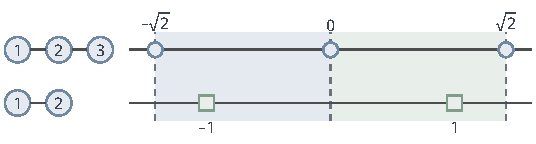
\includegraphics{figures/03-graphs/05-matrices-and-spectra/tikz/adjacency-interlacing-path/figure.pdf}
  \caption{删去三点路径$P_3$的端点$3$得到导出子图$K_2$时的特征值交错关系。上排圆点为$P_3$的邻接特征值$\sqrt2,0,-\sqrt2$，下排方点为二阶主子矩阵$K_2$的特征值$1,-1$，每个新特征值都落在相邻两个原特征值所夹的区间内。}
  \label{fig:adjacency-interlacing-path}
\end{BookInlineFigure}

这正是实对称矩阵的Cauchy交错定理（证明见\BookChapterRef{chap:condition-and-spectral-perturbation}{卷二"条件数与谱扰动"章}）：若$n$阶实对称矩阵$\bm A$的特征值为$\lambda_1\geq\cdots\geq\lambda_n$，其$k$阶主子矩阵$\bm A_0$的特征值为$\mu_1\geq\cdots\geq\mu_k$，则对每个$i=1,\ldots,k$都有$\lambda_i\geq\mu_i\geq\lambda_{i+n-k}$。特别地，取$i=1$可知：任意导出子图$\mathcal G'$的最大邻接特征值都不超过原图的最大邻接特征值，即$\lambda_1(\mathcal G')\leq\lambda_1(\mathcal G)$。需要注意，删顶点得到的是主子矩阵，可直接应用Cauchy交错定理；而单纯删边不删顶点只改变部分非对角元，并非主子矩阵截取。

有了导出子图的最大特征值界，下面同时证明色数$\chi(\mathcal G)$的Wilf上界与Hoffman下界。

\begin{theorem}[色数的谱上下界]
\label{thm:adjacency-chromatic-bounds}
设有限简单无向图$\mathcal G$至少含有一条边，色数为$\chi(\mathcal G)$，其最大与最小邻接特征值分别为$\lambda_1$与$\lambda_n$。则
\begin{equation}
1-\frac{\lambda_1}{\lambda_n}
\leq\chi(\mathcal G)
\leq 1+\lfloor\lambda_1\rfloor.
\label{eq:adjacency-chromatic-bounds}
\end{equation}
\end{theorem}

\begin{proof}
我们先证右侧上界$\chi(\mathcal G)\leq 1+\lfloor\lambda_1\rfloor$（Wilf界），再证左侧下界$\chi(\mathcal G)\geq 1-\lambda_1/\lambda_n$（Hoffman色数界）。

\textbf{第一步（上界证明：导出子图最小度与逆序贪心着色）}：任取原图$\mathcal G$的一个非空导出子图$\mathcal G'$，记其最小顶点度为$\delta(\mathcal G')$，平均度为$\overline d(\mathcal G')$。因为一组数的最小值不超过其平均值，且由定理~\ref{prop:adjacency-degree-bounds}（度下界）与主子矩阵Cauchy交错性质，有不等式链：
\[
\delta(\mathcal G')
\leq\overline d(\mathcal G')
\leq\lambda_1(\mathcal G')
\leq\lambda_1(\mathcal G)=\lambda_1.
\]
由于顶点度是整数，这保证了在$\mathcal G$的任意非空导出子图$\mathcal G'$中，总存在至少一个度不超过$\lfloor\lambda_1\rfloor$的顶点。

据此构造顶点删除序列：在原图$\mathcal G=\mathcal G_n$中选一个度$\leq\lfloor\lambda_1\rfloor$的顶点记为$v_n$并将其删去，得到$n-1$个顶点的导出子图$\mathcal G_{n-1}$；在$\mathcal G_{n-1}$中再选一个在$\mathcal G_{n-1}$内度$\leq\lfloor\lambda_1\rfloor$的顶点记为$v_{n-1}$并删去……如此继续，直到剩下一个顶点$v_1$。现在准备$\lfloor\lambda_1\rfloor+1$种颜色，按相反次序$v_1,v_2,\ldots,v_n$逐个将顶点放回并贪心着色：当放回顶点$v_j$时，它在已放回子图$\mathcal G_j=\{v_1,\ldots,v_j\}$中的邻居个数至多为$\lfloor\lambda_1\rfloor$，这些已着色的邻居至多占用了$\lfloor\lambda_1\rfloor$种颜色，因此在$\lfloor\lambda_1\rfloor+1$种颜色中必有至少一种空闲颜色可供$v_j$使用。故$\chi(\mathcal G)\leq 1+\lfloor\lambda_1\rfloor$。

\textbf{第二步（下界证明：单位根相位消去法）}：由于图至少有一条边，有$\lambda_1>0$；又因$\sum_{i=1}^n\lambda_i=\operatorname{tr}(\bm A)=0$，最小特征值必满足$\lambda_n<0$。

设图$\mathcal G$可以用$k=\chi(\mathcal G)$种颜色正常着色，将颜色编号为$c(u)\in\{0,1,\ldots,k-1\}$（$u\in V$），每条边$\{u,v\}\in E$的两端颜色不同：$c(u)\neq c(v)$。取$k$次本原单位根$\omega=\exp(2\pi\mathrm i/k)$，构造$n\times n$酉对角矩阵
\[
\begin{aligned}
\bm U&=\operatorname{diag}\bigl(\omega^{c(1)},\omega^{c(2)},\ldots,\omega^{c(n)}\bigr),\\
\bm U^*&=\bm U^{-1}=\operatorname{diag}\bigl(\omega^{-c(1)},\omega^{-c(2)},\ldots,\omega^{-c(n)}\bigr).
\end{aligned}
\]
对每个整数$j\in\{0,1,\ldots,k-1\}$，考察共轭矩阵$\bm U^{-j}\bm A\bm U^j$在位置$(u,v)$处的元素：
\[
\bigl(\bm U^{-j}\bm A\bm U^j\bigr)_{u,v}
=a_{u,v}\,\omega^{j(c(v)-c(u))}.
\]
将$j$从$0$到$k-1$对这$k$个矩阵求和：若$\{u,v\}\notin E$，则$a_{u,v}=0$，求和自然为$0$；若$\{u,v\}\in E$，因正常着色要求两端异色，$c(v)-c(u)\not\equiv 0\pmod k$，故公比$\eta=\omega^{c(v)-c(u)}\neq 1$且满足$\eta^k=1$，由等比数列求和公式有
\[
\sum_{j=0}^{k-1}\eta^j=\frac{1-\eta^k}{1-\eta}=0.
\]
这意味着在所有位置$(u,v)$上，$k$个共轭矩阵之和全为零矩阵：
\begin{equation}
\sum_{j=0}^{k-1}\bm U^{-j}\bm A\bm U^j=\bm 0.
\label{eq:adjacency-chromatic-phase-cancellation}
\end{equation}

现在取$\bm A$属于最大特征值$\lambda_1$的实单位特征向量$\bm x\in\mathbb R^n$（$\|\bm x\|_2=1$，$\bm x^\top\bm A\bm x=\lambda_1$），用$\bm x^\top$和$\bm x$夹乘式~\eqref{eq:adjacency-chromatic-phase-cancellation}两端，并令$\bm z^{(j)}=\bm U^j\bm x\in\mathbb C^n$：
\[
0=\sum_{j=0}^{k-1}\bm x^\top\bigl(\bm U^{-j}\bm A\bm U^j\bigr)\bm x
=\bm x^\top\bm A\bm x+\sum_{j=1}^{k-1}(\bm z^{(j)})^*\bm A\bm z^{(j)}.
\]
由于$\bm U^j$的对角元模长全为$1$，每个$\bm z^{(j)}=\bm U^j\bm x$仍是单位向量（$(\bm z^{(j)})^*\bm z^{(j)}=\|\bm x\|_2^2=1$）。在实对称矩阵$\bm A$的正交特征基下展开，任意复单位向量的二次型$(\bm z^{(j)})^*\bm A\bm z^{(j)}$都是特征值$\lambda_1,\ldots,\lambda_n$的凸组合，故不小于最小特征值$\lambda_n$。将$j=0$项的$\lambda_1$与其余$k-1$项的下界$\lambda_n$代入上式：
\[
0\geq\lambda_1+(k-1)\lambda_n.
\]
将负项$-(k-1)\lambda_n$移到左端并同除以$-\lambda_n>0$（注意$\lambda_n<0$），得$k-1\geq\frac{\lambda_1}{-\lambda_n}$，即$k\geq 1-\frac{\lambda_1}{\lambda_n}$。
\end{proof}

我们在完全图$K_n$和五元环$C_5$上检验定理~\ref{thm:adjacency-chromatic-bounds}。对完全图$K_n$，$\lambda_1=n-1,\lambda_n=-1$，下界给出$1-\frac{n-1}{-1}=n$，上界给出$1+\lfloor n-1\rfloor=n$，上下界同时取等，唯一确定$\chi(K_n)=n$。对五元奇环$C_5$，由定理~\ref{prop:adjacency-cycle-spectrum}知$\lambda_1=2$，$\lambda_5=2\cos(4\pi/5)=-\frac{1+\sqrt 5}{2}\approx -1.618$，下界给出
\[
\chi(C_5)\geq 1+\frac{2}{(1+\sqrt 5)/2}=1+\sqrt 5-1=\sqrt 5\approx 2.236.
\]
因为色数必须是整数，向上取整立得$\chi(C_5)\geq 3$；而上界给出$\chi(C_5)\leq 1+2=3$，上下界共同确定$\chi(C_5)=3$。

\subsection{独立数的谱界}
\label{sec:adjacency-hoffman-independence}

在图的正常着色中，涂同一种颜色的所有顶点彼此之间不能有边相连。这种两两互不相邻的顶点子集$S\subseteq V$称为图的\emph{独立集}（independent set），图所含最大独立集的顶点数称为\emph{独立数}（independence number），记为$\alpha(\mathcal G)$。显然，若用$\chi(\mathcal G)$种颜色把$n$个顶点分成$\chi(\mathcal G)$个独立集，每个独立集至多含$\alpha(\mathcal G)$个顶点，必有$n\leq\chi(\mathcal G)\alpha(\mathcal G)$，即$\chi(\mathcal G)\geq n/\alpha(\mathcal G)$。那么，能否直接用邻接谱给出独立数$\alpha(\mathcal G)$的上界？

如果直接取独立集$S$的$0$--$1$指示向量$\bm 1_S$（在$S$内取$1$、在$S$外取$0$），由于$S$内部没有任何边，二次型$\bm 1_S^\top\bm A\bm 1_S=0$恒等于零，从中读不出$|S|$的大小。为了把独立集向外部发出的边数信息引入二次型，同时也为了消去常向量$\bm 1$方向（最大特征值$\lambda_1=d$方向）的分量，我们在$d$正则图上从指示向量$\bm 1_S$中减去它的全图平均值$s/n$（其中$s=|S|$），构造中心化测试向量
\[
\bm x=\bm 1_S-\frac{s}{n}\bm 1.
\]
经过中心化后，$\bm x$在$S$内的$s$个顶点上取正值$1-\frac{s}{n}$，在$S$外的$n-s$个顶点上取负值$-\frac{s}{n}$，且全部$n$个分量之和为零（$\bm 1^\top\bm x=0$，即$\bm x\perp\bm 1$）。此时从$S$连向$V\setminus S$的跨界边两端一正一负，产生负的二次型，正好受最小特征值$\lambda_n$的下方约束。

\begin{theorem}[独立数的Hoffman界]
\label{thm:adjacency-hoffman-independence}
设$\mathcal G$是$n$个顶点的简单$d$正则无向图（$d\geq 1$），最小邻接特征值为$\lambda_n$。则其独立数$\alpha(\mathcal G)$满足
\begin{equation}
\alpha(\mathcal G)\leq n\,\frac{-\lambda_n}{d-\lambda_n}.
\label{eq:adjacency-hoffman-independence}
\end{equation}
\end{theorem}

\begin{proof}
任取$\mathcal G$的一个非空独立集$S\subseteq V$，记$s=|S|\geq 1$。因为$d\geq 1$，图中每个顶点都有边相连，独立集不可能包含全部顶点，故$1\leq s<n$。令$\bm x=\bm 1_S-\frac{s}{n}\bm 1$，则$\bm 1^\top\bm x=s-\frac{s}{n}\cdot n=0$，即$\bm x\in\bm 1^\perp$。

我们分别计算向量$\bm x$的欧氏长度平方$\|\bm x\|_2^2$和二次型$\bm x^\top\bm A\bm x$。首先计算长度平方：因为$\bm 1_S^\top\bm 1_S=s$且$\bm 1_S^\top\bm 1=s$，展开得
\[
\begin{aligned}
\|\bm x\|_2^2
&=\Bigl(\bm 1_S-\frac{s}{n}\bm 1\Bigr)^\top\Bigl(\bm 1_S-\frac{s}{n}\bm 1\Bigr)
=s-2\frac{s}{n}\cdot s+\frac{s^2}{n^2}\cdot n\\
&=s-\frac{s^2}{n}
=s\Bigl(1-\frac{s}{n}\Bigr)>0.
\end{aligned}
\]

再计算二次型$\bm x^\top\bm A\bm x$：利用双线性展开，
\[
\bm x^\top\bm A\bm x
=\bm 1_S^\top\bm A\bm 1_S
-2\frac{s}{n}\bm 1_S^\top\bm A\bm 1
+\frac{s^2}{n^2}\bm 1^\top\bm A\bm 1.
\]
逐项化简右端三项：第一项$\bm 1_S^\top\bm A\bm 1_S=\sum_{u,v\in S}a_{u,v}$等于独立集$S$内部边数的两倍，由于$S$是独立集、内部无边，故$\bm 1_S^\top\bm A\bm 1_S=0$；第二项利用$d$正则图的性质$\bm A\bm 1=d\bm 1$，得$\bm 1_S^\top\bm A\bm 1=d(\bm 1_S^\top\bm 1)=ds$；第三项同样由$\bm A\bm 1=d\bm 1$，得$\bm 1^\top\bm A\bm 1=d(\bm 1^\top\bm 1)=dn$。将三项结果代回，得到
\[
\bm x^\top\bm A\bm x
=0-2\frac{s}{n}(ds)+\frac{s^2}{n^2}(dn)
=-\frac{ds^2}{n}.
\]

现在应用Rayleigh商的最小特征值下界：对任意非零向量$\bm x$，都有$\bm x^\top\bm A\bm x\geq\lambda_n\|\bm x\|_2^2$。将上面算出的$\bm x^\top\bm A\bm x$与$\|\bm x\|_2^2$代入：
\[
-\frac{ds^2}{n}\geq\lambda_n\Bigl(s-\frac{s^2}{n}\Bigr).
\]
在不等式两端同除以正数$s>0$，得
\[
-\frac{ds}{n}\geq\lambda_n-\lambda_n\frac{s}{n}
\quad\Longrightarrow\quad
(d-\lambda_n)\frac{s}{n}\leq -\lambda_n.
\]
因为$d\geq 1$且$\lambda_n<0$，必有$d-\lambda_n>0$。两端同除以$d-\lambda_n$再乘以$n$，即得$s\leq n\frac{-\lambda_n}{d-\lambda_n}$。对最大独立集取$s=\alpha(\mathcal G)$，式~\eqref{eq:adjacency-hoffman-independence}得证。
\end{proof}

从证明过程还可以看到：在$d$正则图上，将式~\eqref{eq:adjacency-hoffman-independence}代入色数与独立数的关系$\chi(\mathcal G)\geq\frac{n}{\alpha(\mathcal G)}$，立得$\chi(\mathcal G)\geq\frac{d-\lambda_n}{-\lambda_n}=1-\frac{d}{\lambda_n}=1-\frac{\lambda_1}{\lambda_n}$，这从独立集视角再次印证了定理~\ref{thm:adjacency-chromatic-bounds}中的Hoffman色数下界。

检验两个例子：对偶数长环$C_{2r}$（$d=2,\lambda_n=-2$）或等侧完全二部图$K_{r,r}$（$d=r,\lambda_n=-r$），Hoffman界给出$\alpha(\mathcal G)\leq n\frac{d}{2d}=\frac{n}{2}$，取二部划分的任一侧即达到等号；对五元环$C_5$（$n=5,d=2,\lambda_5=-\frac{1+\sqrt 5}{2}$），Hoffman界给出$\alpha(C_5)\leq 5\cdot\frac{(1+\sqrt 5)/2}{2+(1+\sqrt 5)/2}=\sqrt 5\approx 2.236$，由于独立数是整数，向下取整得$\alpha(C_5)\leq 2$，任取两个不相邻顶点即达到最大值$2$。

\subsection{同谱图}
\label{sec:adjacency-spectral-information}
\label{sec:adjacency-cospectral-graphs}

综合前面几节的结果，我们可以对“完整邻接谱究竟能告诉我们多少图结构信息”作一全面梳理。

\paragraph{邻接谱确定的图不变量}

给定简单无向图$\mathcal G$的全部$n$个邻接特征值$\lambda_1\ge\cdots\ge\lambda_n$，以下不变量与界可由谱确定（界不等于相应参数的精确值）：
\begin{enumerate}
\item \textbf{顶点数$n$、边数$m$与三角形个数$t_3$}：特征值总个数就是顶点数$n$；由式~\eqref{eq:adjacency-edge-triangle-counts}，$m=\frac12\sum_{i=1}^n\lambda_i^2$，三角形个数$t_3=\frac16\sum_{i=1}^n\lambda_i^3$，以及任意阶$k$步闭行走的总数$\sum_{i=1}^n\lambda_i^k$。
\item \textbf{是否为正则图}：由定理~\ref{prop:adjacency-degree-bounds}，先由二阶谱矩算出平均度$\overline d=\frac1n\sum_{i=1}^n\lambda_i^2$，再检查最大特征值是否满足$\lambda_1=\overline d$。因为常向量$\bm 1$达到最大Rayleigh商$\lambda_1$当且仅当$\bm A\bm 1=\lambda_1\bm 1$（无论图是否连通），所以$\mathcal G$是正则图当且仅当$\lambda_1=\frac1n\sum_{i=1}^n\lambda_i^2$。
\item \textbf{是否为二部图}：由定理~\ref{thm:adjacency-bipartite-spectral-symmetry}的第1条，$\mathcal G$是二部图当且仅当全部特征值关于原点对称（$\lambda_i=-\lambda_{n+1-i},\forall i$）。
\item \textbf{直径、色数与独立数的硬性范围约束}：不同特征值个数给出连通图直径上界$D\leq r-1$，最大与最小特征值给出色数范围$1-\lambda_1/\lambda_n\leq\chi(\mathcal G)\leq 1+\lfloor\lambda_1\rfloor$及正则图独立数上界$\alpha(\mathcal G)\leq n\frac{-\lambda_n}{d-\lambda_n}$。
\end{enumerate}

\paragraph{同谱非同构图}

尽管邻接谱包含丰富的代数信息，但它不能唯一确定图的同构类。如果两张图$\mathcal G$与$\mathcal H$的邻接谱（作为带重数的多重集）完全相同，则称它们为\term{同谱图}（cospectral graphs，或等谱图）。两张同构的图仅相差顶点重新编号（即邻接矩阵相差置换相似变换$\bm P\bm A\bm P^\top$），因此必然同谱；但反过来，存在大量结构截然不同、却拥有完全相同邻接谱的非同构图。

最经典的一对五顶点同谱非同构图如图~\ref{fig:adjacency-cospectral-pair}所示：左图是星图$K_{1,4}$，右图是四元环与一个孤立顶点的不交并$C_4\sqcup K_1$。

\begin{figure}[!htb]
  \centering
  \begingroup
\definecolor{GraphSpectrumNode}{HTML}{E5EAF0}
\definecolor{GraphSpectrumOutline}{HTML}{7188A3}
\definecolor{GraphSpectrumEdge}{HTML}{4C4D4F}
\definecolor{GraphSpectrumText}{HTML}{3B4252}
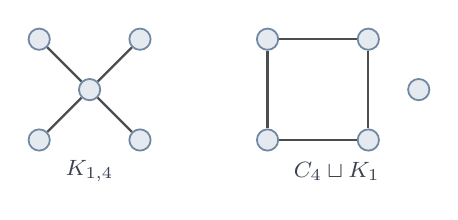
\begin{tikzpicture}[x=8mm,y=8mm,
  vertex/.style={circle,inner sep=0pt,minimum size=2.7mm,
    fill=GraphSpectrumNode,draw=GraphSpectrumOutline,line width=.65pt},
  every path/.style={line width=.8pt},
  title/.style={text=GraphSpectrumText,font=\footnotesize}]
  \begin{scope}
    \node[vertex] (s) at (0,0) {};
    \node[vertex] (l1) at (-.8,.8) {};
    \node[vertex] (l2) at (.8,.8) {};
    \node[vertex] (l3) at (.8,-.8) {};
    \node[vertex] (l4) at (-.8,-.8) {};
    \foreach \v in {l1,l2,l3,l4} {
      \draw[GraphSpectrumEdge] (s) -- (\v);
    }
    \node[title] at (0,-1.3) {$K_{1,4}$};
  \end{scope}
  \begin{scope}[xshift=29mm]
    \node[vertex] (c1) at (-.8,.8) {};
    \node[vertex] (c2) at (.8,.8) {};
    \node[vertex] (c3) at (.8,-.8) {};
    \node[vertex] (c4) at (-.8,-.8) {};
    \node[vertex] at (1.6,0) {};
    \draw[GraphSpectrumEdge] (c1) -- (c2) -- (c3) -- (c4) -- (c1);
    \node[title] at (.3,-1.3) {$C_4\sqcup K_1$};
  \end{scope}
\end{tikzpicture}
\endgroup

  \caption{最小的一对简单无向邻接同谱非同构图。(a) 左图星图$K_{1,4}$由$1$个中心顶点连接$4$个叶子顶点，连通且无环。(b) 右图$C_4\sqcup K_1$由一个四元环与一个孤立顶点组成，不连通且含四元环。两图的邻接谱同为$\{2,0,0,0,-2\}$。}
  \label{fig:adjacency-cospectral-pair}
\end{figure}

利用第~\ref{sec:adjacency-standard-spectra}节的结果立即可以核对两图的谱：左图$K_{1,4}$是$p=1,q=4$的完全二部图，由定理~\ref{prop:adjacency-bipartite-complete-spectrum}，其非零特征值为$\pm\sqrt{1\times 4}=\pm 2$，零特征值重数为$1+4-2=3$，故谱为$\{2,0,0,0,-2\}$；右图$C_4\sqcup K_1$是分块对角矩阵，$C_4$的特征值为$2,0,0,-2$，孤立顶点$K_1$添入一个特征值$0$，合起来的谱也是$\{2,0,0,0,-2\}$。

两张图的全部$5$个特征值一模一样，但它们展示出邻接谱丢失的三项重要结构信息：
\begin{enumerate}
\item \textbf{邻接谱不能判定连通性}：$K_{1,4}$是连通图（一棵树），而$C_4\sqcup K_1$不连通（有$2$个连通分量）。（第~\ref{chap:graph-laplacian-matrix}章将看到，拉普拉斯矩阵的零特征值重数恰等于连通分量个数，从而弥补邻接谱的这一缺陷。）
\item \textbf{邻接谱不能确定度序列}：$K_{1,4}$的度序列是$(4,1,1,1,1)$，而$C_4\sqcup K_1$的度序列是$(2,2,2,2,0)$。虽然两图的度之和都是$2m=8$，但各自的度分布完全不同。
\item \textbf{邻接谱不能确定四元环个数$t_4$}：$K_{1,4}$是树，四元环个数$t_4=0$；而$C_4\sqcup K_1$含有$t_4=1$个四元环。
\end{enumerate}

\paragraph{闭行走的补偿机制}

既然两图同谱，它们的任意阶谱矩$\operatorname{tr}(\bm A^k)=\sum_{i=1}^5\lambda_i^k$都相等，特别是四阶谱矩均为$\operatorname{tr}(\bm A^4)=2^4+(-2)^4=32$。为什么一张没有四元环（$t_4=0$）、另一张有一个四元环（$t_4=1$），四步闭行走的总数却同样是$32$？

用式~\eqref{eq:adjacency-four-cycle-count}把两图的四步闭行走按三类拆开：在星图$K_{1,4}$上，单边往返（第一类）有$2m=8$条，中心点度为$4$、有$\binom{4}{2}=6$对相邻边从而贡献$4\times 6=24$条星形分支往返（第二类），四元环绕行（第三类）为$8\times 0=0$条，合计$8+24+0=32$条。

而在$C_4\sqcup K_1$上，单边往返（第一类）也是$2m=8$条，四环上的$4$个顶点度均为$2$、各有$\binom{2}{2}=1$对相邻边从而只贡献$4\times(1+1+1+1)=16$条第二类行走，但多出的$1$个四元环恰好补上了$8\times 1=8$条第三类绕行，合计同样是$8+16+8=32$条。

可以看到，$K_{1,4}$靠度为$4$的中心节点多产生了$8$条三顶点折返行走，恰好与$C_4\sqcup K_1$沿四元环绕行产生的$8$条行走在求和后相抵。迹算子$\operatorname{tr}(\bm A^k)$只汇总闭行走的总条数，抹去了闭行走究竟来自星形高次度节点还是来自四元环的拓扑细节。

总结而言，邻接谱是图同构的一个必要非充分不变量：若两张图的邻接谱不同，立即可断定它们不同构；但若邻接谱相同，仅凭特征值还不足以确认同构。下一节我们将进一步考察：如果把原图的顶点按对称角色聚合成若干块，用更小的商矩阵代替原邻接矩阵，这种粗粒化的“商谱”又能保留多少谱信息？

\section{商谱}
\label{sec:adjacency-spectral-invariant}

完整邻接谱包含全部$n$个特征值，计算时需要处理$n\times n$矩阵。如果图中的顶点可以按连接角色分成$k$个块（$k\leq n$），使得同一块内的顶点对各个块具有完全相同的邻居计数，那么块与块之间的数值传递就可以用一个规模小得多的$k\times k$矩阵——商矩阵——来完整描述。从商矩阵算出的$k$个特征值称为图的商谱。

商谱并非对原图特征值的粗略数值近似，而是完整邻接谱中对应于“块内取常值”特征方向的精确子集。本节先定义等价划分、商矩阵与商谱，再说明颜色细化算法如何自动生成最粗的等价划分（即公平划分），最后严格证明商矩阵的实谱性质、不变子空间分解以及商谱对完整谱的精确嵌入定理。

\subsection{商矩阵}
\label{sec:adjacency-equitable-quotient}

我们先在四点环加对角边$\{1,3\}$的图上观察一种特殊的分块赋值现象。把度为$3$的两个对角顶点归为第一块$C_1=\{1,3\}$，把度为$2$的另外两个顶点归为第二块$C_2=\{2,4\}$。如图~\ref{fig:adjacency-quotient-block-values}(a)所示，给$C_1$中的顶点$1,3$统一赋读数$a$，给$C_2$中的顶点$2,4$统一赋读数$b$，构成块常值向量$\bm x=(a,b,a,b)^\top$。

现在对$\bm x$施加一次邻接矩阵$\bm A$，逐点查看邻居读数之和：在第一块$C_1$中，顶点$1$的三个邻居是$3\in C_1$（读数$a$）以及$2,4\in C_2$（读数各为$b$），邻居和为$1\cdot a+2\cdot b=a+2b$，顶点$3$的三个邻居是$1\in C_1$和$2,4\in C_2$，邻居和同样为$a+2b$。

在第二块$C_2$中，顶点$2$和顶点$4$的两个邻居都是$1,3\in C_1$（读数各为$a$）、在$C_2$内部没有邻居，故邻居和同为$2\cdot a+0\cdot b=2a$。如图~\ref{fig:adjacency-quotient-block-values}(b)所示，经过邻接矩阵作用后，同一块内的顶点依然保持相同的输出值。第一块统一从$a$更新为$a+2b$，第二块统一从$b$更新为$2a$。这意味着我们无需再逐个追踪全部$4$个顶点，只需用一个$2\times 2$小矩阵就能直接写出两块代表值$(a,b)^\top$的更新规则：
\[
\begin{bmatrix}1&2\\2&0\end{bmatrix}
\begin{bmatrix}a\\b\end{bmatrix}
=\begin{bmatrix}a+2b\\2a\end{bmatrix}.
\]

\begin{BookInlineFigure}
  \centering
  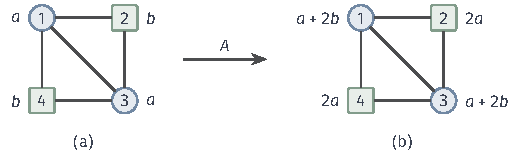
\includegraphics{figures/03-graphs/05-matrices-and-spectra/tikz/adjacency-quotient-block-values/figure.pdf}
  \caption{四点五边图上的块常值赋值与邻接更新。(a) 圆形顶点$C_1=\{1,3\}$统一赋读数$a$，方形顶点$C_2=\{2,4\}$统一赋读数$b$。(b) 经邻接矩阵$\bm A$作用后，$C_1$内每个顶点同取$a+2b$，$C_2$内每个顶点同取$2a$，输出仍为块常值向量。}
  \label{fig:adjacency-quotient-block-values}
\end{BookInlineFigure}

为什么同块内的顶点在乘$\bm A$之后还能保持取值一致？关键在于：同一个块$C_i$中的每一个顶点，落在任意块$C_j$中的邻居个数都是同一个常数。把这一结构条件提炼出来，就得到等价划分与商矩阵的定义。

\begin{definition}[等价划分与商矩阵]
\label{def:adjacency-equitable-partition}
设$\mathcal P=\{C_1,\ldots,C_r\}$是图$\mathcal G=(V,E)$顶点集$V$的一个划分（各块$C_i$非空且互不相交）。若对任意一对下标$i,j\in\{1,\ldots,r\}$（允许$i=j$），块$C_i$中的每一个顶点$u\in C_i$在块$C_j$中所拥有的邻居个数都等于同一个常数$q_{i,j}$（即$\bigl|N(u)\cap C_j\bigr|=q_{i,j}$仅依赖于$i,j$而与$u\in C_i$的具体选取无关），则称$\mathcal P$为图$\mathcal G$的一个\term{等价划分}（equitable partition）。由块间邻居计数$q_{i,j}$排成的$r\times r$矩阵$\bm Q=(q_{i,j})\in\mathbb R^{r\times r}$称为该等价划分的\term{商矩阵}（quotient matrix），$\bm Q$的全部特征值组成的多重集$\operatorname{spec}(\bm Q)$称为对应的\term{商谱}（quotient spectrum）。
\end{definition}

在上面四点五边图的划分$C_1=\{1,3\},C_2=\{2,4\}$中，$q_{1,1}=1,q_{1,2}=2,q_{2,1}=2,q_{2,2}=0$，商矩阵正是
\[
\bm Q=
\begin{bmatrix}
1&2\\
2&0
\end{bmatrix}.
\]
解二次特征方程$\det(\lambda\bm I-\bm Q)=\lambda(\lambda-1)-4=\lambda^2-\lambda-4=0$，立得商谱为
\[
\operatorname{spec}(\bm Q)=\left\{\frac{1+\sqrt{17}}{2},\;\frac{1-\sqrt{17}}{2}\right\}.
\]
原图的完整邻接谱有$4$个特征值，而商谱给出了其中$2$个——那么怎样在一般图上自动寻找这样的划分？另外$2$个特征值又藏在哪里？下面两小节依次回答这两个问题。

\subsection{公平划分}
\label{sec:adjacency-color-refinement-partition}

上一小节从分块矩阵的邻居计数定义了等价划分，但一张图往往存在不止一个等价划分（例如把每个顶点各自单独作为一块，总是包含$n$块的平凡等价划分）。在图算法中，我们希望从没有任何先验区分的统一初色出发，完全依靠图的局部连接结构自动划分出最精简的顶点类别。为此，先从顶点着色（色类）的角度给出公平划分的定义。

\begin{definition}[公平划分]
\label{def:fair-partition}
设图$\mathcal G=(V,E)$的顶点集$V$被划分为$k$个互不相交的非空子集（称为色类或单元）：
\[
V=C_1\cup C_2\cup\cdots\cup C_k.
\]
称该划分为图$\mathcal G$的一个\term{公平划分}（fair partition），如果对任意两个色类$C_i$与$C_j$（$1\leq i,j\leq k$，$i$与$j$可相同也可不同），色类$C_i$中的任意顶点$u\in C_i$在色类$C_j$中的邻居个数都等于一个固定常数$b_{i,j}=\bigl|N(u)\cap C_j\bigr|$，该常数仅取决于色类对$(C_i,C_j)$，而与顶点$u\in C_i$的具体选择无关。
\end{definition}

对比定义~\ref{def:adjacency-equitable-partition}与定义~\ref{def:fair-partition}可以看出，公平划分与等价划分所要求的块间邻居计数条件（$b_{i,j}=q_{i,j}$）在数学上完全一致。本章把这两个名称作为同义表述，不以构造方式区分它们。颜色细化的稳定划分是其中一个特殊成员，须另行证明其最粗性。下面我们依次证明：颜色细化的稳定划分必为公平划分，且它是图上所有等价划分中最粗（块数最少）的那一个。

\subsubsection{颜色细化的稳定划分}
\label{sec:adjacency-color-refinement-stable}

回顾第~\ref{sec:graph-wl-refinement}节的颜色细化算法：初始时（第$0$轮），给图中所有顶点赋同一种初始颜色；在每一轮迭代中，同时检验每个顶点当前的自身颜色以及它在各个当前色类中的邻居个数（合称为该顶点的颜色签名），只有自身颜色相同且对每种颜色的邻居个数也完全相同的顶点，才在下一轮归入同一个新色类，否则就被拆分成不同的色类。由于每次拆分都会使色类的个数严格增加，而$n$个顶点至多只能拆成$n$个单点色类，因此迭代必然在有限步（至多$n-1$轮拆分）内达到稳定状态——即再执行一轮细化，色类划分不再发生任何改变。

图~\ref{fig:adjacency-color-refinement-steps}展示了四点五边图从统一初色出发的颜色细化过程：
\begin{itemize}
\item \textbf{第$0$轮（统一初色）}：如图~\ref{fig:adjacency-color-refinement-steps}(a)所示，四个顶点$\{1,2,3,4\}$全部涂成同一种初始颜色（色$0$）。
\item \textbf{第$1$轮（按度分色）}：如图~\ref{fig:adjacency-color-refinement-steps}(b)所示，统计每个顶点在色$0$中的邻居个数（即顶点度）：顶点$1,3$各有$3$个色$0$邻居（$d=3$），顶点$2,4$各有$2$个色$0$邻居（$d=2$）。于是顶点集分裂为两个色类$C_1=\{1,3\}$（蓝圆）与$C_2=\{2,4\}$（绿方）。
\item \textbf{第$2$轮（核对邻居色分布并稳定）}：如图~\ref{fig:adjacency-color-refinement-steps}(c)所示，分别统计每个顶点在$(C_1,C_2)$两个色类中的邻居个数：$C_1$中的顶点$1$和$3$在$(C_1,C_2)$中的邻居个数同为$(1,2)$；$C_2$中的顶点$2$和$4$在$(C_1,C_2)$中的邻居个数同为$(2,0)$。同一色类内部的所有顶点具有完全相同的邻居计数签名，不再发生任何拆分，算法稳定于划分$\mathcal P_{\mathrm{stable}}=\bigl\{\{1,3\},\{2,4\}\bigr\}$。
\end{itemize}
又如在六元环$C_6$（或任意$d$正则图）上，第$0$轮所有顶点同为色$0$，第$1$轮每个顶点都有$d=2$个色$0$邻居，签名完全相同，从第一步起就不再分裂，稳定划分只有一个色类$C_1=V$。

\begin{BookInlineFigure}
  \centering
  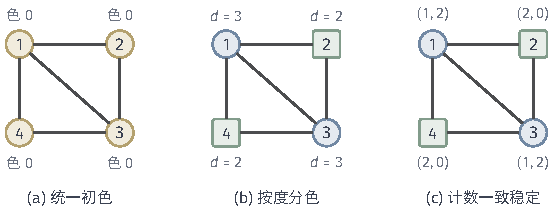
\includegraphics{figures/03-graphs/05-matrices-and-spectra/tikz/adjacency-color-refinement-steps/figure.pdf}
  \caption{四点五边图上的颜色细化稳定过程。(a) 第$0$轮：所有顶点赋统一初色（色$0$）。(b) 第$1$轮：按色$0$邻居数（即顶点度）拆分为度$3$色类$C_1=\{1,3\}$（蓝圆）与度$2$色类$C_2=\{2,4\}$（绿方）。(c) 第$2$轮：$C_1$内各点对$(C_1,C_2)$的邻居计数均为$(1,2)$，$C_2$内各点均为$(2,0)$，划分达到稳定。}
  \label{fig:adjacency-color-refinement-steps}
\end{BookInlineFigure}

下面的定理说明，颜色细化停止（稳定）的那一刻，所得的色类划分自动满足公平划分的定义。

\begin{theorem}[颜色细化的稳定划分是公平划分]
\label{thm:stable-is-equitable}
对任意有限简单无向图$\mathcal G=(V,E)$，从统一初色出发运行颜色细化算法，达到稳定时的色类划分$\mathcal P_{\mathrm{stable}}=\{C_1,\ldots,C_k\}$必为图$\mathcal G$的公平划分。
\end{theorem}

\begin{proof}
设算法在达到稳定划分$\mathcal P_{\mathrm{stable}}=\{C_1,\ldots,C_k\}$后再执行一轮核对。任取两个色类$C_i,C_j\in\mathcal P_{\mathrm{stable}}$，并任取色类$C_i$中的两个顶点$u,v\in C_i$。

因为划分$\mathcal P_{\mathrm{stable}}$已经稳定，再执行一轮颜色细化不会把同属$C_i$的顶点$u$和$v$拆入不同的新色类。根据颜色细化的更新规则，两个同色顶点$u,v$在下一轮保持同色，当且仅当它们在每一个当前色类$C_\ell$（$\ell=1,\ldots,k$）中的邻居个数都分别相等。特别地，取$\ell=j$，即有
\[
\bigl|N(u)\cap C_j\bigr|=\bigl|N(v)\cap C_j\bigr|.
\]
由于$u,v\in C_i$是任意选取的，这说明$C_i$中所有顶点在$C_j$中的邻居个数都等于同一个常数$b_{i,j}$。由定义~\ref{def:fair-partition}，$\mathcal P_{\mathrm{stable}}$是公平划分。
\end{proof}

\subsubsection{最粗等价划分}
\label{sec:adjacency-coarsest-equitable-partition}

既然公平划分与等价划分满足相同的块间邻居计数条件，为什么由颜色细化生成的公平划分在所有等价划分中地位最特殊？答案是：它合并了尽可能多的“结构角色不可区分”的顶点，是图上所有等价划分中最粗（块数最少）的那一个。为了严格表述这一结论，我们先定义两个划分之间的细化偏序关系。

\begin{definition}[划分的细化]
\label{def:partition-refinement}
设$\mathcal P=\{D_1,\ldots,D_r\}$与$\mathcal P'=\{C_1,\ldots,C_k\}$是同一顶点集$V$上的两个划分。若$\mathcal P$中的每一个块$D_a$都完整地包含在$\mathcal P'$的某一个块$C_i$之内（即对每个$a\in\{1,\ldots,r\}$，存在$i\in\{1,\ldots,k\}$使得$D_a\subseteq C_i$），则称划分$\mathcal P$是划分$\mathcal P'$的\term{细化}（refinement），或称$\mathcal P'$比$\mathcal P$更粗（coarser）。若$\mathcal P$是$\mathcal P'$的细化且$\mathcal P\neq\mathcal P'$，则称$\mathcal P$是$\mathcal P'$的严格细化。
\end{definition}

根据定义~\ref{def:partition-refinement}，说$\mathcal P$是$\mathcal P'$的细化，直观上就是指$\mathcal P$可以通过把$\mathcal P'$的某些块进一步切碎得到；等价地，$\mathcal P'$的每一个块$C_i$都恰好是$\mathcal P$中若干个完整块的并集。例如在四点集$\{1,2,3,4\}$上，$\mathcal P=\bigl\{\{1\},\{2\},\{3,4\}\bigr\}$是$\mathcal P'=\bigl\{\{1,2\},\{3,4\}\bigr\}$的细化（将$\{1,2\}$拆成了$\{1\}$和$\{2\}$）；而$\bigl\{\{1,3\},\{2,4\}\bigr\}$不是$\mathcal P'$的细化，因为块$\{1,3\}$横跨了$\mathcal P'$的两个块。在全体划分中，最细的划分是每个顶点各自成一块的单点划分（共$n$块），最粗的划分是全体顶点合成一块的整图划分（仅$1$块）。

现在我们证明：任何等价划分都是颜色细化稳定划分的细化。

\begin{theorem}[统一初色的稳定划分是最粗等价划分]
\label{thm:color-refinement-coarsest}
设$\mathcal P_{\mathrm{stable}}=\{C_1,\ldots,C_k\}$是从统一初色出发运行颜色细化得到的稳定公平划分，$\mathcal P=\{D_1,\ldots,D_r\}$是图$\mathcal G$的任意一个等价划分。则$\mathcal P$必为$\mathcal P_{\mathrm{stable}}$的细化（即$\mathcal P_{\mathrm{stable}}$是图$\mathcal G$最粗的等价划分，并在不计块的排列次序下唯一确定）。
\end{theorem}

\begin{proof}
记$\mathcal P^{(t)}$为颜色细化第$t$轮结束时的色类划分（$t=0,1,2,\ldots$）。我们对轮数$t$作数学归纳法，证明对一切$t\geq 0$，$\mathcal P$都是$\mathcal P^{(t)}$的细化——即颜色细化在任何一轮都不会把等价划分$\mathcal P$的同一个块$D_a$中的两个顶点拆开。

\textbf{归纳基础（$t=0$）}：第$0$轮为统一初色，$\mathcal P^{(0)}=\{V\}$只有一个块。对任意$D_a\in\mathcal P$，显然有$D_a\subseteq V$，故$\mathcal P$是$\mathcal P^{(0)}$的细化。

\textbf{归纳步骤}：假设第$t$轮结束时$\mathcal P$是$\mathcal P^{(t)}$的细化。这意味着$\mathcal P^{(t)}$中的每一个当前色类$C\in\mathcal P^{(t)}$，都恰好是$\mathcal P$中若干个完整块的并集。

现在考察第$t+1$轮的颜色更新。任取$\mathcal P$的一个块$D_a\in\mathcal P$，并任取其中的两个顶点$u,v\in D_a$。由归纳假设，$u$和$v$在第$t$轮属于同一个色类，具有相同的第$t$轮颜色。要证明它们在第$t+1$轮仍然获得相同颜色，只需证明对$\mathcal P^{(t)}$中的任意一个色类$C\in\mathcal P^{(t)}$，$u$和$v$在$C$中的邻居个数相等。

由于$C\in\mathcal P^{(t)}$是$\mathcal P$中若干个互不相交块的并集，设
\[
C=D_{b_1}\cup D_{b_2}\cup\cdots\cup D_{b_s}.
\]
因为$\mathcal P=\{D_1,\ldots,D_r\}$是等价划分（商矩阵记为$q_{a,b}$），块$D_a$中的任意顶点在块$D_{b_\ell}$中的邻居个数都等于固定常数$q_{a,b_\ell}$。由于$D_{b_1},\ldots,D_{b_s}$互不相交，顶点$u\in D_a$在并集$C$中的邻居总数为
\[
\bigl|N(u)\cap C\bigr|
=\sum_{\ell=1}^s\bigl|N(u)\cap D_{b_\ell}\bigr|
=q_{a,b_1}+q_{a,b_2}+\cdots+q_{a,b_s}.
\]
完全相同地，顶点$v\in D_a$在$C$中的邻居总数也为
\[
\bigl|N(v)\cap C\bigr|
=\sum_{\ell=1}^s\bigl|N(v)\cap D_{b_\ell}\bigr|
=q_{a,b_1}+q_{a,b_2}+\cdots+q_{a,b_s}
=\bigl|N(u)\cap C\bigr|.
\]
这对所有色类$C\in\mathcal P^{(t)}$均成立，故$u$和$v$在第$t+1$轮的颜色签名完全一致，仍然留在同一个第$t+1$轮色类中。因此，块$D_a$的全体顶点整体包含在$\mathcal P^{(t+1)}$的某个色类中，即$\mathcal P$也是$\mathcal P^{(t+1)}$的细化。

由数学归纳法，当算法在有限步达到稳定划分$\mathcal P_{\mathrm{stable}}$时，$\mathcal P$仍是$\mathcal P_{\mathrm{stable}}$的细化。
\end{proof}

定理~\ref{thm:color-refinement-coarsest}给出了一个构造结论：我们不需要靠人工猜测去寻找等价划分，只需从统一初色运行确定性的颜色细化算法，就一定能找到全图最粗、块数最少（从而商矩阵维数最小）的规范公平划分$\mathcal P_{\mathrm{stable}}$。当需要判断两张图$\mathcal G$和$\mathcal H$是否可能同构时，可以在它们的不交并$\mathcal G\sqcup\mathcal H$上使用同一套颜色编码同步运行颜色细化：若两图同构，稳定后每个色类在两图中的顶点数$|C_i|$以及块间邻居计数$b_{i,j}$必定完全匹配，导出相同的公平划分商矩阵$\bm Q$；反之，只要色类大小或商矩阵不匹配，立即可断定两图不同构。

\subsection{公平划分的性质}
\label{sec:adjacency-spectral-hierarchy}

找到公平划分$\mathcal P=\{C_1,\ldots,C_k\}$及其$k\times k$商矩阵$\bm Q=(b_{i,j})$之后，一个核心的谱图论问题是：这个小矩阵$\bm Q$的特征值（商谱）与原图$n\times n$邻接矩阵$\bm A$的特征值（完整邻接谱）之间究竟有什么关系？下面我们分三个子小节，通过形式化定理和严格证明逐一揭示商矩阵的实谱性质、块常值不变子空间交织恒等式以及商谱对完整谱的精确嵌入分解，并剖析商谱保留与丢失的结构信息。

\subsubsection{商矩阵的实谱}
\label{sec:adjacency-quotient-real-spectrum}

首先，对给定的图$\mathcal G$，一般的等价划分可以有很多个，各自导出不同阶数的商矩阵；但根据定理~\ref{thm:color-refinement-coarsest}，从统一初色出发由颜色细化生成的公平划分$\mathcal P=\{C_1,\ldots,C_k\}$作为最粗等价划分是唯一确定的。因此，在不计$k$个色类排列顺序（即对$\bm Q$的行和列同时施加相同置换$\bm P\bm Q\bm P^\top$）的意义下，公平划分导出的商矩阵$\bm Q$及其商谱$\operatorname{spec}(\bm Q)$是图$\mathcal G$唯一确定的代数不变量。

其次，观察商矩阵$\bm Q=(b_{i,j})$的形式：虽然原图的邻接矩阵$\bm A$是对称矩阵，但商矩阵$\bm Q$通常不是对称矩阵。例如在三点路径$1\text{--}2\text{--}3$上，公平划分将两个度为$1$的端点归为第一块$C_1=\{1,3\}$（$|C_1|=2$），将度为$2$的中心点归为第二块$C_2=\{2\}$（$|C_2|=1$）。此时，$C_1$中的每个端点在$C_2$中只有$b_{1,2}=1$个邻居，而$C_2$中的中心点在$C_1$中却有$b_{2,1}=2$个邻居，商矩阵为
\[
\bm Q=\begin{bmatrix}0&1\\2&0\end{bmatrix},\qquad b_{1,2}=1\neq 2=b_{2,1}.
\]
既然$\bm Q$不对称，它的特征值会不会出现复数？能不能对角化？下面的定理通过“双向计数跨块边数”证明：商矩阵$\bm Q$虽然自身未必对称，但通过块大小对角矩阵作一次对角相似变换，就能变成实对称矩阵。

\begin{theorem}[商矩阵的实谱性质]
\label{thm:quotient-matrix-real-spectrum}
设$\mathcal P=\{C_1,\ldots,C_k\}$是有限简单无向图$\mathcal G=(V,E)$的一个公平划分（或任意等价划分），商矩阵为$\bm Q=(b_{i,j})\in\mathbb R^{k\times k}$，记块大小对角矩阵为
\[
\bm D_C=\operatorname{diag}\bigl(|C_1|,|C_2|,\ldots,|C_k|\bigr).
\]
则块大小与商矩阵满足对称平衡恒等式
\begin{equation}
|C_i|\,b_{i,j}=|C_j|\,b_{j,i}\quad(\forall\,1\leq i,j\leq k),
\qquad\text{即}\qquad
\bm D_C\bm Q=\bm Q^\top\bm D_C.
\label{eq:adjacency-quotient-symmetry}
\end{equation}
进一步，矩阵
\[
\widetilde{\bm Q}=\bm D_C^{1/2}\bm Q\bm D_C^{-1/2}
\]
是$k\times k$实对称矩阵。因此，商矩阵$\bm Q$在实数域$\mathbb R$上可对角化，其全部$k$个特征值均为实数。
\end{theorem}

\begin{proof}
任取两个色类$C_i$与$C_j$（当$i=j$时$|C_i|b_{i,i}=|C_j|b_{j,i}$恒成立；以下设$i\neq j$），我们从左右两侧分别计算横跨在$C_i$与$C_j$之间的无向边总数$e(C_i,C_j)$：从$C_i$一侧计数，$C_i$中共有$|C_i|$个顶点，由公平划分定义，其中每一个顶点在$C_j$中都恰好有$b_{i,j}$个邻居，故跨块边总数为$e(C_i,C_j)=|C_i|\,b_{i,j}$；从$C_j$一侧计数，$C_j$中共有$|C_j|$个顶点，其中每一个顶点在$C_i$中都恰好有$b_{j,i}$个邻居，故同一批跨块边的总数又等于$e(C_i,C_j)=|C_j|\,b_{j,i}$。两边相等即得$|C_i|\,b_{i,j}=|C_j|\,b_{j,i}$。注意到$(\bm D_C\bm Q)_{i,j}=|C_i|b_{i,j}$，而$(\bm Q^\top\bm D_C)_{i,j}=(\bm Q^\top)_{i,j}|C_j|=b_{j,i}|C_j|$，故矩阵等式$\bm D_C\bm Q=\bm Q^\top\bm D_C$成立，式~\eqref{eq:adjacency-quotient-symmetry}得证。

由于每个色类$C_i$非空，$|C_i|\geq 1>0$，对角矩阵
\[
\bm D_C^{1/2}=\operatorname{diag}\bigl(\sqrt{|C_1|},\ldots,\sqrt{|C_k|}\bigr)
\]
及其逆矩阵$\bm D_C^{-1/2}$均为实可逆对角矩阵。对$\bm D_C\bm Q=\bm Q^\top\bm D_C$两端左乘$\bm D_C^{-1/2}$、右乘$\bm D_C^{-1/2}$，得到
\[
\bm D_C^{1/2}\bm Q\bm D_C^{-1/2}
=\bm D_C^{-1/2}\bm Q^\top\bm D_C^{1/2}
=\bigl(\bm D_C^{1/2}\bm Q\bm D_C^{-1/2}\bigr)^\top,
\]
这证明了$\widetilde{\bm Q}=\bm D_C^{1/2}\bm Q\bm D_C^{-1/2}$是实对称矩阵（其第$(i,j)$个元素为$b_{i,j}\sqrt{|C_i|/|C_j|}=b_{j,i}\sqrt{|C_j|/|C_i|}$）。

由实对称矩阵谱定理，$\widetilde{\bm Q}$有$k$个实特征值和一组标准正交实特征向量基$\tilde{\bm y}_1,\ldots,\tilde{\bm y}_k$。因为$\bm Q=\bm D_C^{-1/2}\widetilde{\bm Q}\bm D_C^{1/2}$与实对称矩阵$\widetilde{\bm Q}$相似，二者具有完全相同的特征多项式与实特征值，且$\bm y_r=\bm D_C^{-1/2}\tilde{\bm y}_r$（$r=1,\ldots,k$）构成$\bm Q$在$\mathbb R^k$中的一组线性无关实特征向量基，故$\bm Q$在$\mathbb R$上可对角化。
\end{proof}

\subsubsection{商谱嵌入}
\label{sec:adjacency-quotient-spectrum-embedding}

为了把$k\times k$商矩阵$\bm Q$与$n\times n$邻接矩阵$\bm A$连接起来，我们引入公平划分$\mathcal P=\{C_1,\ldots,C_k\}$的\emph{块指示矩阵}（characteristic matrix）$\bm S\in\mathbb R^{n\times k}$：其第$j$列就是色类$C_j$在顶点空间$\mathbb R^n$中的$0$--$1$指示向量$\bm 1_{C_j}$：
\[
S_{u,j}=(\bm 1_{C_j})_u=
\begin{cases}
1,& u\in C_j,\\
0,& u\notin C_j,
\end{cases}
\qquad 1\leq u\leq n,\;1\leq j\leq k.
\]
由于$C_1,\ldots,C_k$互不相交且非空，$\bm S$的各列在不同坐标集合上取$1$，满足
\[
\bm S^\top\bm S=\operatorname{diag}\bigl(|C_1|,\ldots,|C_k|\bigr)=\bm D_C,
\]
故$\bm S$列满秩（$\operatorname{rank}\bm S=k$）。

对任意块读数向量$\bm y=(y_1,\ldots,y_k)^\top\in\mathbb R^k$，左乘$\bm S$得到的$n$维向量
\[
\bm S\bm y=\sum_{j=1}^k y_j\,\bm 1_{C_j}\in\mathbb R^n
\]
在每个色类$C_j$的所有顶点上统一取常数值$y_j$。因此，$\bm S$的列空间
\[
\mathcal W=\operatorname{col}(\bm S)=\bigl\{\bm S\bm y:\bm y\in\mathbb R^k\bigr\}\subseteq\mathbb R^n
\]
是由全体“在每个色类内部取常值”的顶点向量组成的$k$维子空间，称为划分$\mathcal P$的\term{块常值子空间}（block-constant subspace）。而$\mathcal W$在$\mathbb R^n$中的正交补空间
\[
\mathcal W^\perp
=\ker(\bm S^\top)
=\Bigl\{\bm z\in\mathbb R^n:\bm 1_{C_j}^\top\bm z=\sum_{u\in C_j}z_u=0,\;\forall\,j=1,\ldots,k\Bigr\}
\]
则由全体“在每一个色类内部分量之和均为零”的顶点向量组成，维数为$n-k$。

下面的定理揭示了公平划分的本质代数特征：块常值子空间$\mathcal W$及其正交补$\mathcal W^\perp$都是邻接矩阵$\bm A$的不变子空间。

\begin{theorem}[商矩阵的交织恒等式]
\label{thm:quotient-intertwining}
设$\mathcal P=\{C_1,\ldots,C_k\}$是图$\mathcal G=(V,E)$的顶点集划分，$\bm S\in\mathbb R^{n\times k}$为其块指示矩阵。则$\mathcal P$是以$\bm Q=(b_{i,j})\in\mathbb R^{k\times k}$为商矩阵的公平划分（等价划分），当且仅当邻接矩阵$\bm A$与商矩阵$\bm Q$满足交织恒等式
\begin{equation}
\bm A\bm S=\bm S\bm Q.
\label{eq:adjacency-quotient-intertwining}
\end{equation}
在此条件下，块常值子空间$\mathcal W=\operatorname{col}(\bm S)$及其正交补空间$\mathcal W^\perp=\ker(\bm S^\top)$均为$\bm A$的不变子空间（即$\bm A\mathcal W\subseteq\mathcal W$且$\bm A\mathcal W^\perp\subseteq\mathcal W^\perp$）。
\end{theorem}

\begin{proof}
首先证明$\mathcal P$为商矩阵是$\bm Q$的公平划分当且仅当$\bm A\bm S=\bm S\bm Q$。任取顶点$u\in V$（设$u$属于色类$C_i$）和列下标$j\in\{1,\ldots,k\}$，分别计算式~\eqref{eq:adjacency-quotient-intertwining}左右两端在位置$(u,j)$处的元素。左端$\bm A\bm S$的第$j$列为$\bm A\bm 1_{C_j}$，其在顶点$u$处的元素为
\[
(\bm A\bm S)_{u,j}=(\bm A\bm 1_{C_j})_u=\sum_{v\in C_j}a_{u,v}=\bigl|N(u)\cap C_j\bigr|,
\]
即顶点$u$在色类$C_j$中的邻居个数；右端$\bm S\bm Q$在位置$(u,j)$处的元素为$\sum_{\ell=1}^k S_{u,\ell}\,b_{\ell,j}$，因为$u\in C_i$，只有$\ell=i$时$S_{u,i}=1$、其余$\ell\neq i$时$S_{u,\ell}=0$，故
\[
(\bm S\bm Q)_{u,j}=b_{i,j}.
\]
对比左右两端可知：$(\bm A\bm S)_{u,j}=(\bm S\bm Q)_{u,j}$对所有$u\in C_i$和所有$i,j$成立，当且仅当对任意$u\in C_i$都有$|N(u)\cap C_j|=b_{i,j}$，这正是定义~\ref{def:fair-partition}中公平划分的充要条件。

接下来证明$\mathcal W$与$\mathcal W^\perp$均为$\bm A$的不变子空间。一方面，对任意块常值向量$\bm w=\bm S\bm y\in\mathcal W$（$\bm y\in\mathbb R^k$），由交织恒等式~\eqref{eq:adjacency-quotient-intertwining}，有
\[
\bm A\bm w=\bm A(\bm S\bm y)=(\bm A\bm S)\bm y=\bm S(\bm Q\bm y)\in\operatorname{col}(\bm S)=\mathcal W,
\]
故$\bm A\mathcal W\subseteq\mathcal W$。另一方面，对任意$\bm z\in\mathcal W^\perp$和任意$\bm w\in\mathcal W$，由于$\bm A$是实对称矩阵（$\bm A^\top=\bm A$）且已证$\bm A\bm w\in\mathcal W$，有
\[
\langle\bm A\bm z,\bm w\rangle
=(\bm A\bm z)^\top\bm w
=\bm z^\top(\bm A\bm w)
=\langle\bm z,\bm A\bm w\rangle=0.
\]
这说明$\bm A\bm z$与$\mathcal W$中的一切向量正交，即$\bm A\bm z\in\mathcal W^\perp$，故$\bm A\mathcal W^\perp\subseteq\mathcal W^\perp$。定理得证。
\end{proof}

由定理~\ref{thm:quotient-intertwining}的交织恒等式$\bm A\bm S=\bm S\bm Q$，我们可以立即导出商谱与原图完整邻接谱之间的精确嵌合定理。

\begin{theorem}[商谱嵌入定理]
\label{thm:quotient-spectrum-inclusion}
设$\mathcal P=\{C_1,\ldots,C_k\}$是有限简单无向图$\mathcal G=(V,E)$的一个公平划分（或任意等价划分），块指示矩阵为$\bm S\in\mathbb R^{n\times k}$，商矩阵为$\bm Q\in\mathbb R^{k\times k}$。则：
\begin{enumerate}
\item 若$\bm y\in\mathbb R^k\setminus\{\bm 0\}$是商矩阵$\bm Q$属于特征值$\lambda$的特征向量（$\bm Q\bm y=\lambda\bm y$），则块常值向量$\bm S\bm y\in\mathcal W\setminus\{\bm 0\}$是原图邻接矩阵$\bm A$属于同一特征值$\lambda$的特征向量；
\item 按代数重数计，商矩阵的商谱$\operatorname{spec}(\bm Q)$等于$\bm A$限制在块常值子空间$\mathcal W$上的特征值多重集$\operatorname{spec}(\bm A|_{\mathcal W})$，从而完整包含在原图邻接谱中：
\[
\operatorname{spec}(\bm Q)\subseteq\operatorname{spec}(\bm A),\qquad
\operatorname{spec}(\bm A)=\operatorname{spec}(\bm Q)\,\cup\,\operatorname{spec}(\bm A|_{\mathcal W^\perp}),
\]
其中$\bm A$限制在正交补$\mathcal W^\perp$上的$n-k$个特征值$\operatorname{spec}(\bm A|_{\mathcal W^\perp})$称为该划分下的\term{剩余谱}（residual spectrum）；
\item 原图的最大邻接特征值$\lambda_1(\bm A)$必然包含在商谱$\operatorname{spec}(\bm Q)$中。
\end{enumerate}
\end{theorem}

\begin{proof}
\textbf{第1条与第2条}：因为$\bm S^\top\bm S=\bm D_C$可逆，线性映射$\bm S\colon\mathbb R^k\to\mathcal W$是双射（线性同构）：当$\bm y\neq\bm 0$时必有$\bm S\bm y\neq\bm 0$。若$\bm Q\bm y=\lambda\bm y$，由定理~\ref{thm:quotient-intertwining}的$\bm A\bm S=\bm S\bm Q$，立得
\[
\bm A(\bm S\bm y)=\bm S(\bm Q\bm y)=\bm S(\lambda\bm y)=\lambda(\bm S\bm y),
\]
即$\bm S\bm y\in\mathcal W$是$\bm A$属于特征值$\lambda$的特征向量。更进一步，式~\eqref{eq:adjacency-quotient-intertwining}表明线性算子$\bm A|_{\mathcal W}\colon\mathcal W\to\mathcal W$在基$\{\bm 1_{C_1},\ldots,\bm 1_{C_k}\}$下的表示矩阵恰好就是$\bm Q$，因此$\bm A|_{\mathcal W}$的特征多项式与$\bm Q$的特征多项式恒同，$\operatorname{spec}(\bm A|_{\mathcal W})=\operatorname{spec}(\bm Q)$（含重数）。又因$\mathbb R^n=\mathcal W\oplus\mathcal W^\perp$是$\bm A$的两个正交不变子空间的直和，在由$\mathcal W$的一组正交特征基与$\mathcal W^\perp$的一组正交特征基拼成的全空间正交基下，$\bm A$呈分块对角形$\operatorname{diag}(\bm A|_{\mathcal W},\bm A|_{\mathcal W^\perp})$，故完整邻接谱$\operatorname{spec}(\bm A)$等于商谱$\operatorname{spec}(\bm Q)$与剩余谱$\operatorname{spec}(\bm A|_{\mathcal W^\perp})$的并集。

\textbf{第3条（$\lambda_1(\bm A)\in\operatorname{spec}(\bm Q)$）}：由定理~\ref{thm:quotient-matrix-real-spectrum}，实对称矩阵$\widetilde{\bm Q}=\bm D_C^{1/2}\bm Q\bm D_C^{-1/2}$逐元素非负，与$\bm Q$（从而与$\bm A|_{\mathcal W}$）具有相同的最大特征值$\mu_{\max}=\lambda_1(\bm Q)$。在原图$\mathcal G$中取一个达到全图最大邻接特征值$\lambda_1(\bm A)$的连通分量$V_0$；当$V_0$至少含两个顶点时应用定理~\ref{thm:adjacency-perron}，单点分量则直接取其指示向量。由此存在一个在$V_0$上各分量严格为正、在$V\setminus V_0$上为$0$的非负特征向量$\bm p\in\mathbb R^n$，满足$\bm A\bm p=\lambda_1(\bm A)\bm p$。

而在正交补$\mathcal W^\perp$中，任意向量$\bm z\in\mathcal W^\perp$在每个色类$C_j$内的分量之和均为零（$\sum_{u\in C_j}z_u=0$）。考察$\bm p$在块常值子空间$\mathcal W$上的正交投影$\bm p_{\mathcal W}$：它在每个色类$C_j$上取该块内$\bm p$分量的平均值$\bar p_j=\frac{1}{|C_j|}\sum_{u\in C_j}p_u\geq 0$。因为$\bm p$在$V_0$上严格为正，至少有一个色类的平均值$\bar p_j>0$，故$\bm p_{\mathcal W}\neq\bm 0$。又因为$\mathcal W$与$\mathcal W^\perp$是$\bm A$的正交不变子空间，$\bm A\bm p=\lambda_1(\bm A)\bm p$两边向$\mathcal W$作正交投影即得$\bm A\bm p_{\mathcal W}=\lambda_1(\bm A)\bm p_{\mathcal W}$。这证明了$\bm p_{\mathcal W}\in\mathcal W\setminus\{\bm 0\}$是$\bm A|_{\mathcal W}$属于$\lambda_1(\bm A)$的特征向量，故$\lambda_1(\bm A)\in\operatorname{spec}(\bm A|_{\mathcal W})=\operatorname{spec}(\bm Q)$。
\end{proof}

我们回到四点五边图（图~\ref{fig:adjacency-quotient-block-values}），用定理~\ref{thm:quotient-spectrum-inclusion}把它的$4$个特征值完整拆解为商谱与剩余谱两部分。首先，在块常值子空间$\mathcal W$中（$k=2$个特征值），公平划分为$C_1=\{1,3\},C_2=\{2,4\}$，$\mathcal W=\operatorname{span}\{(1,0,1,0)^\top,(0,1,0,1)^\top\}$是二维的，前面已由$2\times 2$商矩阵$\bm Q=\bigl[\begin{smallmatrix}1&2\\2&0\end{smallmatrix}\bigr]$算出两个商特征值
\[
\lambda_1=\frac{1+\sqrt{17}}{2}\approx 2.562,\qquad
\lambda_4=\frac{1-\sqrt{17}}{2}\approx -1.562,
\]
全图的最大特征值$\lambda_1=(1+\sqrt{17})/2$确实落在了商谱中。

其次，在正交补$\mathcal W^\perp$中（$n-k=2$个剩余特征值），向量要求在$C_1=\{1,3\}$内分量之和为零（$z_1+z_3=0$）且在$C_2=\{2,4\}$内分量之和也为零（$z_2+z_4=0$），因此$\mathcal W^\perp$直接由两个块内反对称差向量张成：
\[
\bm z_1=(1,0,-1,0)^\top,\qquad
\bm z_2=(0,1,0,-1)^\top.
\]
将邻接矩阵$\bm A$分别作用在这两个向量上：对$\bm z_1=(1,0,-1,0)^\top$，顶点$1$读到邻居$3$的$-1$，顶点$3$读到邻居$1$的$+1$，顶点$2,4$同时读到邻居$1$的$+1$与邻居$3$的$-1$（相加为$0$），故$\bm A\bm z_1=(-1,0,1,0)^\top=-\bm z_1$，直接给出第一个剩余特征值$\lambda_3=-1$；对$\bm z_2=(0,1,0,-1)^\top$，顶点$1$和$3$各自同时连接邻居$2$（读数$+1$）和邻居$4$（读数$-1$），正负抵消为$0$，顶点$2$和$4$只连接读数为$0$的顶点$1,3$，邻居和也为$0$，故$\bm A\bm z_2=\bm 0=0\cdot\bm z_2$，给出第二个剩余特征值$\lambda_2=0$。将商谱$\bigl\{\frac{1+\sqrt{17}}{2},\frac{1-\sqrt{17}}{2}\bigr\}$与剩余谱$\{0,-1\}$合并，就精确得到了四点五边图的全部$4$个邻接特征值：
\[
\operatorname{spec}(\bm A)=\left\{\frac{1+\sqrt{17}}{2},\;0,\;-1,\;\frac{1-\sqrt{17}}{2}\right\}.
\]

\subsubsection{商谱的局限}
\label{sec:adjacency-quotient-information}

定理~\ref{thm:quotient-spectrum-inclusion}的正交分解$\mathbb R^n=\mathcal W\oplus\mathcal W^\perp$揭示了商矩阵$\bm Q$与商谱$\operatorname{spec}(\bm Q)$能够捕捉什么、又会遗漏什么。根据定义~\ref{def:fair-partition}，商矩阵$\bm Q=(b_{i,j})$只记录色类$C_i$中的每个顶点落在色类$C_j$中的邻居个数$b_{i,j}$。只要块间与块内的邻居计数$b_{i,j}$给定，邻接矩阵$\bm A$在块常值子空间$\mathcal W$上的作用就完全固定，从而唯一决定了包括全图最大特征值$\lambda_1(\bm A)$在内的全部$k$个商特征值。

然而，给定每个顶点在同色类内部的邻居个数$b_{i,i}$（或两个色类之间的邻居个数$b_{i,j}$），并不能唯一决定这些边在色类内部究竟是如何连接的。例如在一个包含$6$个顶点的色类中，要求每个顶点恰好有$b_{1,1}=2$个同色邻居，这$6$个顶点既可以首尾相连围成一个连通的六元环$C_6$，也可以拆成两个互不相连的三角形$2C_3=C_3\sqcup C_3$。任何保持各块邻居计数$b_{i,j}$不变的内部重连，都不会改变公平划分和商矩阵$\bm Q$；它们对邻接矩阵$\bm A$的影响完全局限在块内零和的正交补空间$\mathcal W^\perp$上，只可能改变该子空间上的限制算子及其剩余谱，商谱保持不变；不同限制算子仍可能同谱。

图~\ref{fig:adjacency-c6-vs-2c3-quotient}具体展示了六点环$C_6$与两个不相交三角形$2C_3$的这一对比。由于两张图都是$6$个顶点的$2$正则图，从统一初色出发运行颜色细化时，每个顶点都有$2$个同色邻居，第一轮就不发生任何分裂，稳定后的公平划分都只有$k=1$个色类$C_1=V$，导出的$1\times 1$商矩阵同为$\bm Q=(2)$，商谱同为$\operatorname{spec}(\bm Q)=\{2\}$（对应一维常向量子空间$\mathcal W=\operatorname{span}\{\bm 1\}$）。

但在五维正交补空间$\mathcal W^\perp=\bm 1^\perp$上，两张图的内部连接差异使剩余谱完全不同：连通六元环$C_6$的完整邻接谱为$\{2,1,1,-1,-1,-2\}$，扣去商谱$\{2\}$后的$5$个剩余特征值为$1,1,-1,-1,-2$。

而不连通图$2C_3$由两个三角形拼成，完整邻接谱为$\{2,2,-1,-1,-1,-1\}$，其$5$个剩余特征值为$2,-1,-1,-1,-1$（其中落在$\mathcal W^\perp$中的第二个特征值$2$直接反映了两个连通分量的存在，而这一信息在缩减为商矩阵$\bm Q=(2)$时已经丢失）。

\begin{BookInlineFigure}
  \centering
  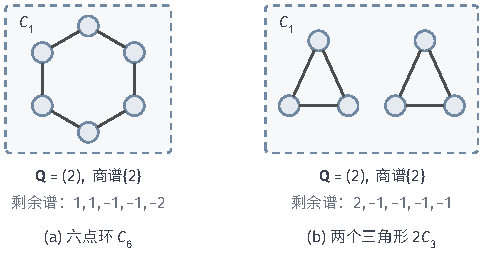
\includegraphics{figures/03-graphs/05-matrices-and-spectra/tikz/adjacency-c6-vs-2c3-quotient/figure.pdf}
  \caption{商谱相同而剩余谱不同的两张$6$点$2$正则图。在统一初色下，两图的公平划分都只有单一色类$C_1=V$（虚线框，$k=1$），商矩阵均为$\bm Q=(2)$，商谱均为$\{2\}$。(a) 六点环$C_6$在$\mathcal W^\perp$上的$5$个剩余特征值为$1,1,-1,-1,-2$。(b) 两个三角形$2C_3$在$\mathcal W^\perp$上的$5$个剩余特征值为$2,-1,-1,-1,-1$。}
  \label{fig:adjacency-c6-vs-2c3-quotient}
\end{BookInlineFigure}

最后，把$C_6$与$2C_3$的例子同第~\ref{sec:adjacency-cospectral-graphs}小节的五顶点同谱图$K_{1,4}$与$C_4\sqcup K_1$（图~\ref{fig:adjacency-cospectral-pair}）放在一起，就能看清颜色细化（公平划分）与完整邻接谱在区分非同构图时的互补关系。

一方面，商谱只是完整邻接谱在$\mathcal W$上的子集：像$C_6$与$2C_3$这样颜色细化完全无法区分（公平划分与商谱均相同）的两张正则图，仍有可能依靠$\mathcal W^\perp$上的剩余谱被完整邻接谱区分开。

另一方面，完整邻接谱也并不能涵盖颜色细化的全部信息：$K_{1,4}$与$C_4\sqcup K_1$拥有完全相同的完整邻接谱$\{2,0,0,0,-2\}$，但颜色细化在第一轮按顶点度分色时，就会把$K_{1,4}$拆成度为$4$和度为$1$的两个色类（大小$1+4$，商矩阵$\bigl(\begin{smallmatrix}0&4\\1&0\end{smallmatrix}\bigr)$），而把$C_4\sqcup K_1$拆成度为$2$和度为$0$的两个色类（大小$4+1$，商矩阵$\bigl(\begin{smallmatrix}2&0\\0&0\end{smallmatrix}\bigr)$），从而将这两张同谱图区分开。完整邻接谱与公平划分各自从特征值多重集和局部度传递层次刻画了图的结构。

\section{本章小结}
\label{sec:adjacency-matrix-summary}

邻接矩阵的$k$次幂在位置$(u,v)$记录从$u$到$v$的$k$步行走条数。对角元之和（迹）给出闭行走总数。实对称性保证迹等于特征值$k$次幂之和，这就是谱矩。

典型图的谱可以直接构造。完全图利用常向量与零和向量，完全二部图利用两侧对称，环利用周期边界的单位根，路径利用零端边界的正弦模式。笛卡儿积图的特征值等于各因子特征值之和。正则图的常向量特征值等于度，补图的谱由此换算。

谱本身具有结构性质。连通图的最大特征值是单根，有严格正的Perron向量。它夹在平均度和最大度之间，连通正则图中两端同时取等。删边或删正权顶点不增大谱半径。二部图的谱关于零对称，非二部图没有这种对称。

完整谱与图结构的关系体现在两个方面。一方面，谱记录了图的宏观代数特征：低阶谱矩确定边数和三角形数，极端特征值限制直径、独立数和色数。另一方面，谱丢失了同构信息：$K_{1,4}$和$C_4\sqcup K_1$有相同谱却不同构，不同来源的闭行走在求和后互相补偿。

更粗的商谱进一步缩减信息。等价划分把图缩成商矩阵，颜色细化给出最粗的等价划分。商谱保留了块间连接密度的框架，丢失了块内的微观差异——颜色细化分不出的两张图，完整谱仍可以不同。

下一章把邻接作用换成沿边差分再加权汇总，得到拉普拉斯矩阵。常值函数的沿边差分全为零，因此零空间直接揭示连通分量——恰好弥补邻接谱在这方面的缺失。

